\chapter{Introduction and Literature Review} % Chapter Title
\label{LR}

\section{The atmosphere}
\label{LR:Atmos}
  % Overarching description of atmosphere
  The atmosphere is made up of gases held to the earth's surface by gravity. 
  These gases undergo transport on all scales, from barbecue smoke being blown about the garden, to smoke plumes from forest fires travelling across the world and depositing in the Antarctic snow.
  They take part in innumerable chemical reactions along the way, largely driven by solar input and interactions with each other.
  Many gases are emitted into the atmosphere by soil, trees, factories, cars, seas and oceans.
  They are also deposited back to the surface both directly and in rainfall.
  
  % Air
  The atmosphere is made up of nitrogen (N$_2$: $\sim 78\%$), oxygen (O$_2$: $\sim 21\%$), and argon (Ar: $\sim 1\%$), along with water (H$_2$O) and \textit{trace gases} (those that make up less than 1\% of the atmosphere).
  Water (H$_2$O) ranges from $0.001$ to $1\%$ depending on evaporation and precipitation.
  Beyond these major constituents the atmosphere has a vast number of trace gases, including carbon dioxide (CO$_2$: $\sim 0.4\%$), ozone (O$_3$: $.000001$ to $0.001\%$), and methane (CH$_4$: $\sim 0.4\%$) \parencite[][Ch. 2]{BrasseurJacob2017}.
  Trace gases in the atmosphere can have a large impact on conditions for life on earth.
  They react in complex ways with other elements (anthropogenic and natural), affecting all surface ecosystems upon which life depends.
  
  One important trace gas is ozone (O$_3$), which affects climate, human health, and ecosystem productivity.
  This thesis will focus on ozone in the troposphere, which is relatively uncertain over Australia.
  
  Ozone in the lower atmosphere is a serious hazard that causes health problems \parencite{Hsieh2013}, damages agricultural crops worth billions of dollars \parencite{Avnery2011,Yue2017}, and increases the rate of climate warming \parencite{IPCC_2013_chap8}.
  Around 5 to 20 percent of all air pollution related deaths are due to ozone \parencite{Monks2015}, roughly .8 million deaths per year \parencite{Lelieveld2013}.
  In the short term, ozone concentrations of $\sim$50-60~ppbv over eight hours or $\sim$80~ppbv over one hour are agreed to constitute a human health hazard \parencite{Ayers2006,Lelieveld2009}. 
  Long term exposure causes problems with crop loss and ecosystem damage \parencite{Emberson2003}, and concentrations may get worse in the future \parencite{Lelieveld2009, Stevenson2013}.
  Further tropospheric ozone enhancements are projected to drive reductions in global crop yields equivalent to losses of up to \$USD$_{2000}$ 35 billion (equivalent to US dollars in the year 2000) per year by 2030 \parencite{Avnery2011}, along with detrimental health outcomes equivalent to $\sim$\$USD$_{2000}$11.8 billion per year by 2050 \parencite{Selin2009}.
  Recently \textcite{Yue2017} showed that the net effect of near-surface ozone on is a $\sim 14\%$ decrease in net primary productivity in China.
  They state that reducing this decrease by $\sim 70\%$ before 2030 would require drastic measures.
  
  
  \subsection{Structure}
  \label{LR:Atmos:Struct}
    
    Most of the atmosphere ($\sim 85\%$) is within 10~km of the earth's surface.
    This is due to air pressure, which decreases logarithmically with altitude.
    Any entity is subjected to the weight of all the air above it, and the density of the atmosphere is driven by this pressure.
    
    The atmosphere extends above the earth's surface to the edges of space. 
    This is split into various layers, defined by the \textit{lapse rate}: the decrease in temperature (\textit{T}) with increasing altitude (\textit{z}), or $\frac{-\textrm{d}T}{\textrm{d}z}$.
    Figure \ref{LR:Atmos:Struct:Fig_atmos_layers} shows the pressure and temperature profiles against altitude through the atmosphere.
    The first layer is the troposphere, which extends to roughly 10~km and is characterised by positive lapse rate (or decreasing temperature with altitude).
    At the top of the troposphere (the tropopause) the temperature stops decreasing, and then the stratosphere is defined by a negative lapse rate.
    This is due to UV radiation being absorbed by ozone, and leads to a very vertically stable environment.
    
    \begin{figure}
      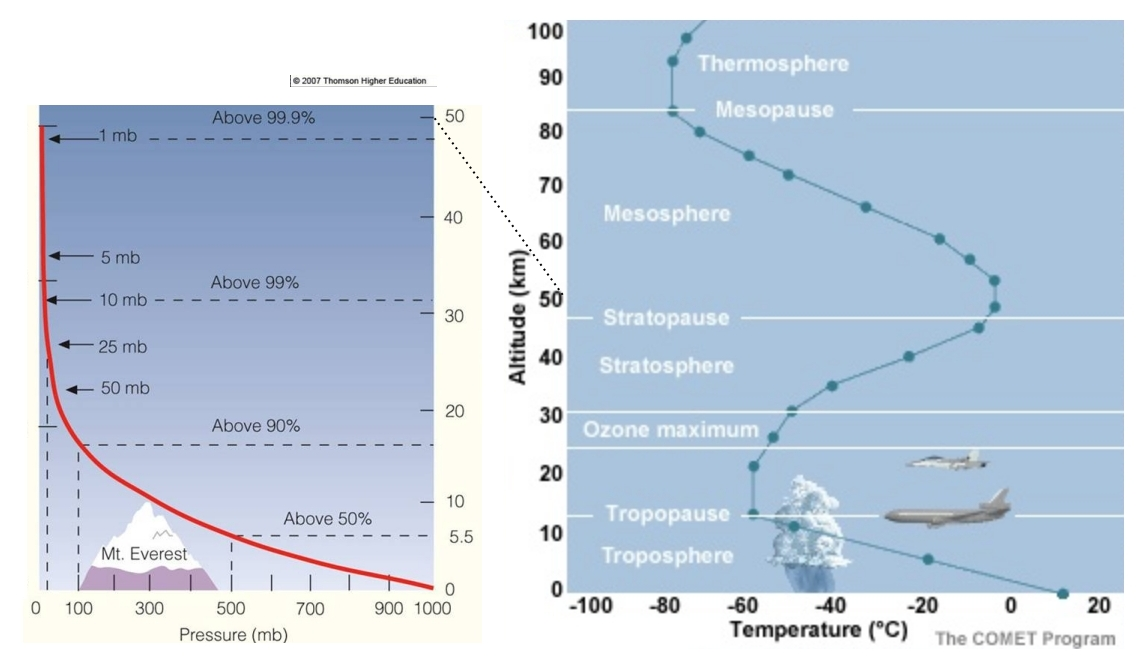
\includegraphics[width=\textwidth]{Figures/Atmos_Temp_Press.jpg}
      \caption{%
        Pressure (red) logarithmically decreasing, shown with percentage of atmosphere below at several points.
        Temperature (green) changes throughout the atmosphere.
        Figure edited from \url{https://climate.ncsu.edu/edu/Structure}.
      }
      \label{LR:Atmos:Struct:Fig_atmos_layers}
    \end{figure}
    
    
    
    % Boundary layer
    In addition to these atmospheric layers, the troposphere can be subset into the \textit{boundary layer} and the \textit{free troposphere}.
    The \textit{boundary layer} is the lowest layer and involves increased atmospheric mixing due to ground heating and friction effects.
    It generally extends anywhere from 200 - 1000~m, above which the ground effects have fewer direct impacts.
    The \textit{free troposphere} is the remainder of the troposphere and is more affected by transport, both horizontally and from the stratosphere.
    
    
  % Chemistry
  \subsection{Composition and chemistry}
  \label{LR:Atmos:Chem}
        
    There are a myriad of trace gases in the atmosphere, emitted by plants, animals, earth, and water. 
    These gases react with one another and over time they either deposit back onto the earth or form more stable compounds such as CO$_2$.
    Oxidation and photolysis (the process of being broken apart by photons) are the two main processes whereby compounds are broken down in the atmosphere.
    
    
    % Oxidation and Radicals
    %\subsubsection{Hydroxyl radicals}
    %\label{LR:Atmos:Chem:radicals}
    OH and HO$_2$ concentrations largely determine the oxidative capacity of the atmosphere.
    Concentration of the OH radical drives many processes in the atmosphere, especially during the day when photolysis of ozone produces OH \parencite{Atkinson2000}.
    OH is a key species which reacts with nearly all the organic compounds in the troposphere, with only a few exceptions \parencite{Atkinson2000}.
    %The exceptions are chlorofluorocarbons (CFCs), and Halons not containing H atoms \parencite{Atkinson2000}.
    Over land, isoprene (C$_5$H$_8$) and monoterpenes (C$_{10}$H$_{16}$) account for 50\% and 30\% of the OH reactivity respectively \parencite{Fuentes2000}.
    
    Since radicals are involved in all oxidative chemistry in the atmosphere it is important for models to accurately represent them (eg. \textcite{Travis2014}).
    This is difficult as they are coupled with so many other species and measurements of OH are not readily available on a global scale.
    In the late '90s it was thought that OH radicals were formed exclusively from photolysis of O$_3$, HONO, HCHO, and other carbonyls (R$_2$C=O) \parencite{Atkinson2000}.
    It has been shown since that OH is recycled in various processes.
    Isoprene (C$_5$H$_8$) was thought to be a sink of OH until it was shown by \textcite{Paulot2009b} that the radicals are recycled.
    This recycling process is discussed in more detail in section \ref{LR:VOCs:IsopCascade}.
    
    Ozone is an important precursor to OH, as excited oxygen atoms (O(${}^1$D)) are created through its photolysis, which then go on to react with water to form OH, as shown in this reaction sequence \parencite{Atkinson2000, AtkinsonArey2003}:
    \begin{equation}
      \begin{aligned}
        O_3+\text{hv}     & \to  O_2 + O({}^1D)   && (\lambda \le 350 \text{nm}) \\%
        O({}^1D)+M        & \to  O({}^3P) + M     && (M=N_2, O_2)               \\%
        O({}^3P)+O_2 + M  & \to  O_3 + M          &&                           \\%
        O({}^1D)+H_2O     & \to  2OH              &&                            \\%
      \end{aligned}
      \label{LR:Atmos:Chem:eqn_O3toOH}
    \end{equation}
    Where $hv$ represents radiation and M is an inert molecule.
    This shows that some of the O$({}^1D)$ recycles back to ozone, while some forms OH.
    %\textcite{AtkinsonArey2003} discuss the relative rates of these reactions.
      
  \subsection{Radiative Forcing}
    \label{LR:VOCs:IsopCascade:RF}
    
    One of the larger uncertainties in atmospheric modelling is how particles in the atmosphere affect radiative forcing.
    For 12 years it has been understood that aerosols overall cool the atmosphere, with smaller particles having a larger effect as they matching the wavelengths of visible light \parencite{Kanakidou2005}.
    Aerosol products from gas phase emissions (or the children thereof) play an indirect and complex role in cloud properties, with a net cooling effect (\textcite{Kanakidou2005}, \textcite[Chapter 7,8]{IPCC_AR5_WG1}).
    
    Transport and indirect effects complicate matters further, with cloud creation and modification of cloud properties being quite difficult to accurately predict.
    In the third IPCC report \parencite{IPCC2001}, the uncertainty involved if OA forcing was a factor of 3 times the estimated effect. 
    This has since been improved however OA and cloud formation still remains a large uncertainty in more recent IPCC reports \parencite{IPCC_Chapter2}.
    Figure \ref{LR:VOCs:IsopCascade:RF:fig_IPCC_RF_AR4} shows the radiative forcing (RF) of various atmospheric constituents, it is clear that OA uncertainty dominates.
    Figure \ref{LR:VOCs:IsopCascade:RF:fig_IPCC_RF_AR5} shows the same summary updated in chapter 8 of the fifth report, where the SOA uncertainty remains large.
    
    \begin{figure}
      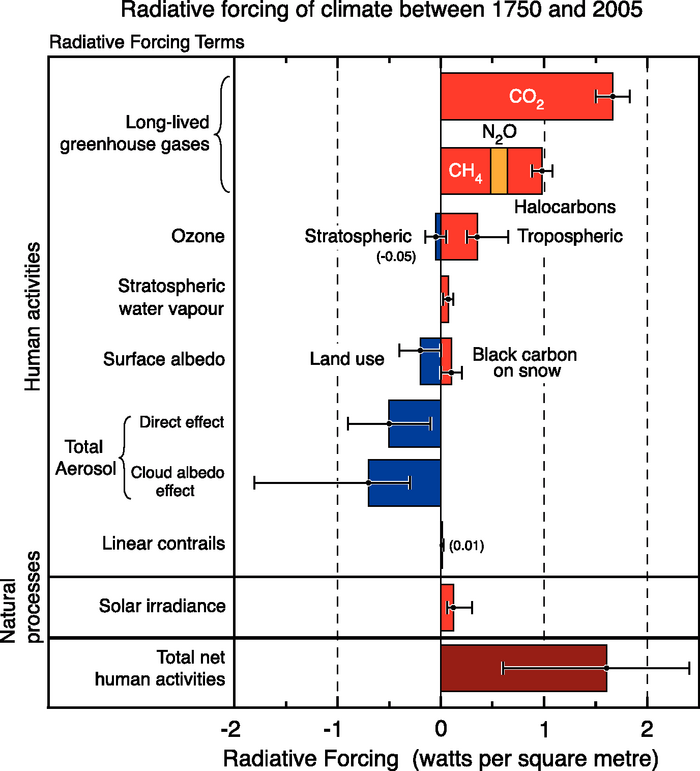
\includegraphics[width=\textwidth]{Figures/IPCC_WG1AR4_RFSummary.png}
      \caption{%
        The overall radiative forcings and uncertainties of several atmospheric constituents
        This is an image taken from \textcite{IPCC_Chapter2}, found at \url{https://www.ipcc.ch/publications_and_data/ar4/wg1/en/faq-2-1.html}.}
     \label{LR:VOCs:IsopCascade:RF:fig_IPCC_RF_AR4}
    \end{figure}
    
    \begin{figure}
      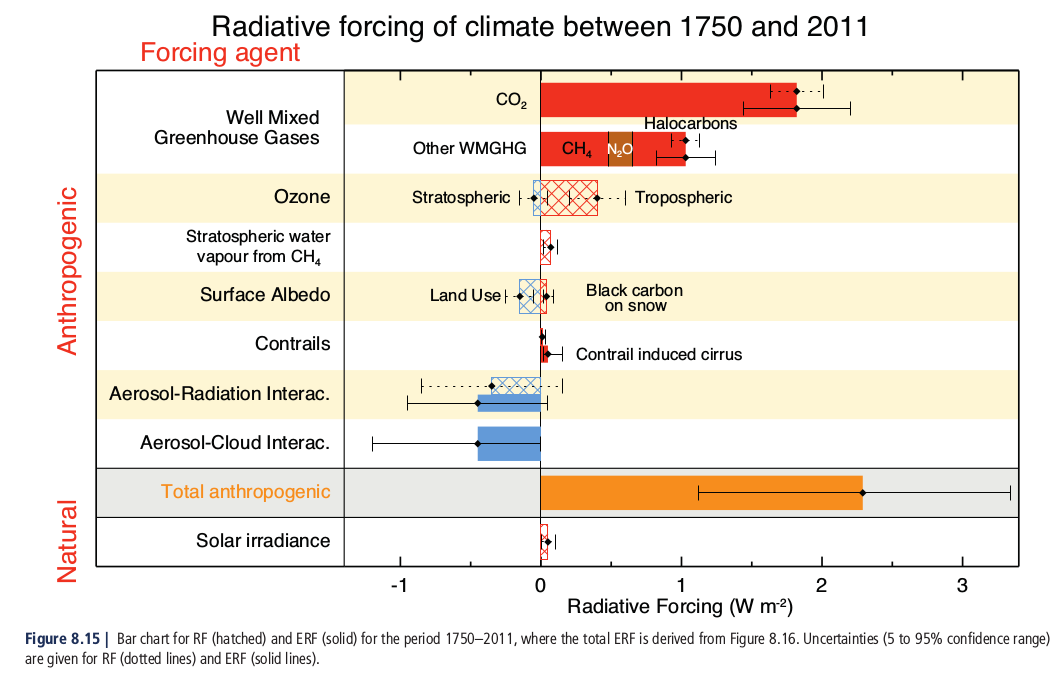
\includegraphics[width=\textwidth]{Figures/IPCC_WG1AR5_RFSummary.png}
      \caption{%
        The overall radiative forcings and uncertainties of several atmospheric constituents
        This is an image taken from \textcite{IPCC_AR5_WG1}, chapter 8.}
      \label{LR:VOCs:IsopCascade:RF:fig_IPCC_RF_AR5}
    \end{figure}    
    
    It has been known for quite a while that our understanding of VOC emissions needs to be improved in order to better capture radiative forcing \parencite{Kanakidou2005}.
    VOC emissions affect ozone along with several atmospheric parameters which directly and indirectly alter radiative forcing rates \parencite[eg.][]{Arneth2008}
    VOCs can lead to changes in cloud formation, as nucleation can arise from the subsequent SOA.
    \textcite{Kanakidou2005} concluded that it is very likely that organics contribute to particle growth and formation rates, and that satellite datasets should be used to improve emissions inventories.
    This is even more important in Australia where VOCs are so poorly represented by contemporary modelling \parencite{Emmerson2016}.

\section{Ozone}
\label{LR:O3}
  
  Ozone (O$_3$) is an important greenhouse gas and oxidant.
  It is mostly located in the stratosphere and prevents much of the shorter wavelength (UV) solar radiation from reaching the earth's surface.
  Ozone in the troposphere is less beneficial, leading to health issues, radiative forcing \parencite{Stevenson2013}, and crop death.
  Understanding and accurately portraying ozone concentrations in the troposphere is important to allow accurate predictions of future climate.
  This will become even more important as projections of future climate changes suggest altered vertical mixing rates, ultra violet index and ozone RF \parencite{Hegglin2009}.
  
  \subsection{Stratospheric ozone}
  
    %Structure of ozone layer chapman eqn etc.
    In the stratosphere ozone production is driven by the Chapman mechanism, as high energy radiation (with wavelengths $\lambda<242$~nm) photolyses the molecular oxygen (O$_2$) in the atmosphere \parencite[][Chapter 3, section 2]{BrasseurJacob2017}.
    The Chapman mechanism involves several reactions which lead to rough equilibrium of O, O$_2$, O$_3$ and pressure, as follows:
    \begin{equation}
      \begin{aligned}
        \text{O}_2 + hv              & \to \text{O}+\text{O}     && \lambda < 242 \text{nm} \\
        \text{O}+\text{O}_2+\text{M} & \to \text{O}_3+\text{M}   &&    \\
        \text{O}_3 + hv              & \to \text{O}+\text{O}_2   && \lambda < 1180 \text{nm} \\
        \text{O} + \text{O}_3        & \to \text{O}_2+\text{O}_2 &&       \\
      \end{aligned}
      \label{LR:O3:eqn_Chapman}
    \end{equation}
    The high energy photons ($\lambda < 242$~nm) are present from the top of the atmosphere but are mostly removed before reaching the troposphere as their energy is used to split the O$_2$ molecules.
    The lifetime of O against loss by O$_2$ is less than a second in the troposphere, and produced O$_3$ quickly returns to O and O$_2$, as low energy ($\lambda < 1180$~nm) photons and M are abundant.
    The reduced light penetration towards the surface, in addition to the logarithmic increase in atmospheric pressure (which affects M abundance) drives the vertical profile of ozone into what is called the \textit{ozone layer}.
    This is a layer of relative ozone abundance within the stratosphere.
    The Chapman mechanism requires radiation so only takes place during the daytime, during the night this process slows to a halt, and the ozone concentrations remain stable unless pollution intrudes \parencite[Chapter 10]{Jacob_1999_book}.
  
    
    % Measurements
    Since the Montreal Protocol on Substances that Deplete the Ozone Layer was established in August 1987, and ratified in August 1989, several satellites and many measurement stations were set up to monitor ozone in the stratosphere.
    However, in the southern hemisphere there are relatively few records of ozone \parencite{Huang2017}.
    This affects our ability to accurately determine sources of ozone in the troposphere, with current southern hemisphere trends lacking full explanation \parencite{Zeng2017}. 
  
  \subsection{Tropospheric ozone}
    Figure \ref{LR:O3:fig_YoungOzoneSummary}, copied from \textcite{Young2018}, shows summary of the major processes and emissions affecting tropospheric ozone.
    This thesis involves improving the highly uncertain natural emissions of volatile organic compounds (VOCs) from Australia, and estimating impacts from STEs.
    
    \begin{figure}
      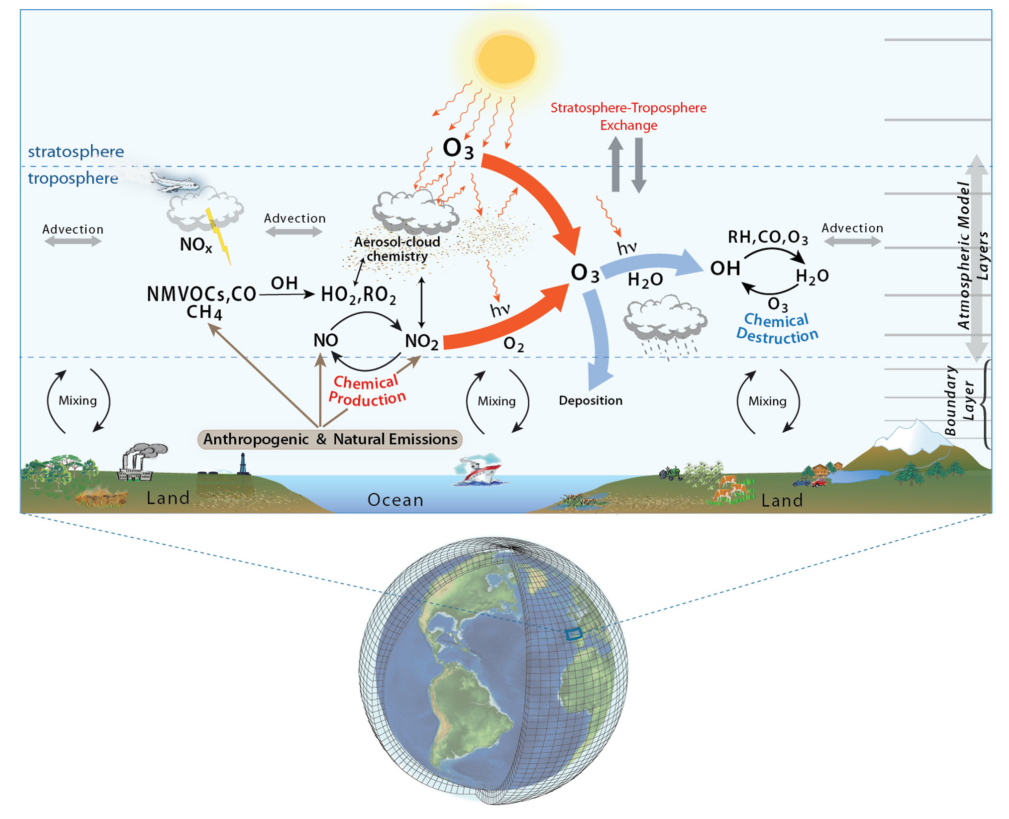
\includegraphics[width=\textwidth]{Figures/Young2018_Figure1.png}
      \caption{%
        Tropospheric ozone processes, Figure 1 in \textcite{Young2018}.
        DOI: https://doi.org/10.1525/elementa.265.f1
      }
      \label{LR:O3:fig_YoungOzoneSummary}
    \end{figure}
  
    %What drives ozone in the troposphere? 
    Generally there are two main drivers of tropospheric ozone concentrations; transport from the stratosphere and chemical production due to emissions of precursors. 
    Tropospheric ozone is regulated by NO and NO$_2$ concentrations, which form an equilibrium \parencite{Cape2008,Young2018}.
    At small to medium scales, pyrogenic (fire) and anthropogenic (man-made) emissions can be important.
    Smoke plumes from biomass burning can carry ozone precursors, creating higher ozone concentrations downwind of the plume's source.
    Emissions of precursors from large cities (primarily traffic and power production) can impact ozone concentrations.
    These impacts are not always straightforwards due to the nonlinear relationship between ozone and its precursors.
    
    % Nox's role 
    NO$_X$ ($\equiv $ NO$_2 +$ NO) is another important chemical family in the atmosphere which interacts with ozone and regulates the atmospheric oxidative capacity.
    NO$_X$ or VOC emissions affect the tropospheric ozone equilibrium and can lead to enhanced ozone formation, shown in figure \ref{LR:O3:fig_YoungOzoneSummary}.
    NO$_X$ compounds are short lived, with emissions (Power generation and combustion transport) being the main driver of concentrations \parencite{Delmas1997}.
    NO$_X$ is removed primarily by conversion to nitric acid (HNO$_3$) followed by wet or dry deposition \parencite{Ayers2006}.
    
    % photoequilibrium of ozone and NOx with and without VOC influence
    NO$_X$ and O$_3$ relative concentrations during the day are regulated by the following reactions \parencite{Sillman1999,Atkinson2000}:
    \begin{equation}
      \begin{aligned}
        NO + O_3         & \to NO_2 + O_2      && \\%
        NO_2 + \text{hv} & \to NO + O({}^3P)   && \\%
        O({}^3P) + O_2   & \to O_3 			 && \\%
      \end{aligned}
      \label{LR:Atmos:Chem:eqn_NOandO3}
    \end{equation}
    This process with and without the influence of VOCs (panel A and B respectively) is summarised in figure \ref{LR:O3:fig_Atkinson_photoequilibrium}.
    
    \mypicw{0.7\textwidth}
      {Figures/Atkinson2000_photoequilibrium.png}
      {Figure showing NO, NO$_2$, and Ozone photoequilibrium cycle with and without (B, A respectively) influence from VOCs. Figure copied from \textcite{Atkinson2000}.}
      {\label{LR:O3:fig_Atkinson_photoequilibrium}}
    
    
    
    % With the NO$_3$ reactions occuring within seconds.
    %%NO_2 + O_3       & \to NO_3 + O_2      && \\%
    %%NO_3 + \text{hv} & \to NO + O_2        && (\sim 10\%)  \\%
    %%NO_3 + \text{hv} & \to NO_2 + O({}^3P) && (\sim 90\%)  \\%
  
  \subsection{Stratosphere to troposphere transport}
    \label{LR:O3:STT}
    %% STT
    Historically, ozone transported down from the stratosphere was thought to contribute 10-40~ppb to tropospheric ozone levels, matching tropospheric production \parencite{Atkinson2000, Stohl2003}.
    The proportion of tropospheric ozone due to transport from the stratosphere was revised down to around 10\% over the years as measurement and modelling campaigns improved our understanding of global scale transport, mixing, and chemistry \parencite{Guenther2006,Monks2015}.
    Intrusions of stratospheric air into the troposphere are often called Stratosphere to Troposphere Transport (STT) events.
    Although most tropospheric ozone comes from production, STT enhancements of ozone are measurable and can be regionally important \parencite[eg.][]{Jacobson2000,Lelieveld2009,Kuang2017}, and upper tropospheric ozone can be transported long distances \parencite{Cooper2004}.
    An analysis of the Atmospheric Chemistry and Climate Model Inter-comparison Project (ACCMIP) simulations by \textcite{Young2013} found STT is responsible for $540\pm140$~Tg yr$^{-1}$, equivalent to $\sim$11\% of the tropospheric ozone column \parencite{Monks2015}.
    
    
    Ozone transported to the troposphere from the stratosphere can occur through diffusion (relatively slowly) or direct mixing (as STT).
    STT often occur as tongues of stratospheric air descend and get disconnected from the stratosphere, potentially due to low pressure systems and jet streams \parencite{Sprenger2003}.
    Recently global chemical transport models (CTMs) have been used to trace how much ozone is being transported to the troposphere in this manner.
    There are a few methods of doing this, such as modeling ozone formed in (and transported from) the stratosphere \parencite{Ojha2016}.
    Model based estimates require validation against actual measurements, such as those from ozonesondes or satellites.
    %Hegglin, M. I., and T. G. Shepherd (2009), Large climate-induced changes in ultraviolet index and stratosphere-to-troposphere ozone flux, Nature Geosci, 2(10), 687 \selectlanguage{english}691, doi:10.1038/NGEO604.
    \textcite{Hegglin2009} estimate that climate change will lead to increased STT.
    They posit that this is due to an acceleration in the Brewer Dobson circulation; which is the global scale model of transport of air in the troposphere and stratosphere.
    They estimate $\sim 30$, and $\sim 121$~Tg yr$^{-1}$ increases by 2095 (relative to 1965) in the southern and northern hemispheres respectively, up by 23\% globally.
    
    \textcite{Liu2017} examine southern hemispheric ozone and the processes which control its inter-annual variability (IAV).
    IAV is the standard deviation of ozone anomalies from the monthly mean.
    They show that ozone transported from the stratosphere plays a major role in the upper troposphere, especially over the southern Indian ocean during austral winter.
    STT mostly impacts the upper troposphere, although some areas are impacted right down to the surface.
    \textcite{Kuang2017} found a measurable impact of STT ozone enhancement in the south east US using several different instruments. 
    They also show how ozone depends on both the local topography, weather systems, and trace gases emitted and transported into the region.
    \textcite{Liu2017} examined modelled tropospheric ozone sensitivity to various meteorological parameters.
    %They showed that ozone at 430~hPa (roughly 6~km altitude) is mostly stratospheric in September over 20$^{\circ}$S to 60$^{\circ}$S at all longitudes.
    They found tropospheric ozone sensitivity to emissions from South America (0--20$^{\circ}$S, 72.5--37.5$^{\circ}$W), southern Africa (5--10$^{\circ}$S, 12-38$^{\circ}$E), and South to South east Asia (70-125$^{\circ}$E, 10$^{\circ}$S--40$^{\circ}$N).
    In the US recent work by \textcite{Lin2015} suggests that intrusions during spring are increasing surface ozone levels.
    They recommend improvements to understanding of the frequency and cause of STT are needed effectively implement air quality standards.
    Recently, modelled ozone concentrations has been shown to be most sensitive to NO$_X$ sources (such as lightning and car exhaust emissions) and isoprene emissions \parencite{Christian2018}.
    
    % Uncertainties?
    
    
  \subsection{Chemical production}
    
    Ozone produced in the troposphere from precursors and radiation drive ozone levels, especially in the lower (near-surface) troposphere.
    The main processes involved are shown in figure \ref{LR:O3:fig_YoungOzoneSummary}, with ozone regulated by reactions \ref{LR:Atmos:Chem:eqn_NOandO3}.
    As discussed above STTs source $\sim 11\%$ of the tropospheric column of ozone, with the remainder produced photochemically \parencite{Monks2015}.
    A recent summary by \textcite{Young2018} estimates ozone production and loss in the troposphere to be $\sim$4900\tgpyr, and $\sim$4500\tgpyr respectively. 
    These numbers are at the global scale, and it should be noted that meteorology and topography can play massive roles due to large spatial variability in ozone \parencite[eg.][]{Kuang2017}.
    
    Tropospheric ozone concentrations require climate and ozone precursor emissions; including NO, NO$_2$, CO, and VOCs such as HCHO \parencite{Atkinson2000, Young2013, Marvin2017}.
    Ozone predictions are uncertain and changing climate affects transport, deposition, destruction, and plant based precursor emissions.
    All of these processes are tightly coupled and difficult to accurately model, as they depend on uncertain assumptions such as CO$_2$ dependency \parencite{Young2013}.
    Even with all the work done over the prior decades there remain large uncertainties about ozone precursors in the troposphere \parencite{Mazzuca2016}.
    
    
    %% How VOCs and Ozone interact:
    Ozone is formed in the troposphere through oxidation of VOCs (described in Section \ref{LR:VOCs}) in the presence of NO$_X$.
    Net formation or loss of O$_3$ is determined by interactions between VOCs, NO$_X$, and HO$_X$, and is a complicated system of positive and negative feedbacks \parencite{Atkinson2000}.
    Figure \ref{LR:VOCs:fig_NOXVOCOzone} shows an example of this non-linear relationship between NO$_X$, VOCs, and ozone production as modelled in \textcite{Mazzuca2016}.
    This non-linear relationship is examined in more detail in the following section (\ref{LR:VOCs}).
    Recently the relationship has been examined on the intradiel timescale showing that ozone production can be more or less sensitive to VOCs at different hours \parencite{Mazzuca2016}.
    This shows how important it is to correctly determine the precursors concentrations in order to estimate ozone levels and production.
    
    \begin{figure}
      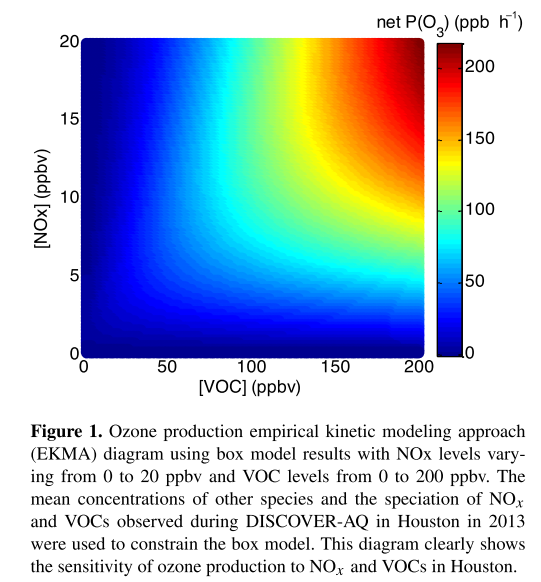
\includegraphics[width=.75\textwidth]{Figures/Mazzuca2016_NOxVOCOzone.png}
      \caption{Ozone production rate dependent on NO$_X$ and VOC concentrations \parencite{Mazzuca2016}.}
      \label{LR:VOCs:fig_NOXVOCOzone}
    \end{figure}
    
    % Loss pathways
    Tropospheric ozone is lost via chemical destruction and dry deposition, estimated to be $4700\pm700$ Tg yr$^{-1}$ and $1000\pm200$ Tg yr$^{-1}$, respectively \parencite{Stevenson2006,Young2018}.
    The main loss channel is through equation \ref{LR:Atmos:Chem:eqn_O3toOH}, where photolysis and collisions (increasing with pressure) create OH from the O$_3$.
    

\section{Volatile Organic Compounds}
\label{LR:VOCs}

  % What they are
  The least well understood precursors to tropospheric ozone production belong to a class of organic compounds.
  Organic compounds are members of a large class of chemicals whose molecules contain carbon, with the exception of a few compounds such as carbides, carbonates, and simple oxides of carbon and cyanide.
  Organic compounds can be categorised based on their vapour pressure, which is the tendency of a liquid or solid to vaporise.
  Compounds with high vapour pressures at standard temperature are classed as volatile, evaporating at low temperatures.
  Plants contain tens of thousands of organic compounds, with fewer than 40 having high enough volatility to be emitted \parencite{Guenther2000}.
  Gas phase emissions with higher vapour pressures can be oxidised into lower vapour pressure products which will partition between gas and particle phase, often called semi or non-volatile. 
  
  % Volatility of organic compounds, and their other attributes
  Atmospheric organic compounds are legion and differ by orders of magnitude with respect to their fundamental properties, such as volatility, reactivity, and cloud droplet formation propensity, etc.
  Volatile organic compounds (VOCs) have vapour pressure greater than $10^{-5}$~atm, and are mostly generated naturally by plants, which emit around 1000\tgpyr \parencite{Guenther1995, Glasius2016}.
  Due to their high volatility these compounds generally exist in the gas phase.
  Organic compounds with a lower volatility are classed as semi-volatile (SVOCs: vapour pressure between $10^{-5}$ and $10^{-11}$~atm) are found in both gas and particle phase depending on temperature and pressure.
  Organic compounds with even lower vapour pressure are generally found in the particle phase in aerosol particulate matter \parencite{Glasius2016}.
  Understanding the drivers of trends in biogenic VOC emissions (BVOCs) is required in order to estimate future carbon fluxes, changes in the water cycle, ozone production, air quality, and other climate responses \parencite{Yue2015}.
  In the last 20 years anthropogenic emissions of VOCs have been increasing while biogenic VOC emissions have decreased, due to rapid economic growth and lower annual temperatures \parencite{Stavrakou2014, Kwon2017}.
  
  Methane (CH$_4$) is one of the more abundant VOCs, however it is often classified separately and compared against non-methane VOCs (NMVOCs).
  NMVOCs include alkanes, alkenes, and aromatic hydrocarbons, with isoprene (an alkene) being the most abundant \parencite{Guenther1995}.
  Methane is relatively long lived (years) and is well mixed in the atmosphere while other VOC levels are spatially diverse due to their shorter lifetimes.
  In this thesis I work towards a better understanding of the isoprene emissions coming from Australia.

  %% What do VOCs do?
  VOCs are an important driver of atmospheric processes, especially near forests.
  VOCs are broken down into HCHO, O$_3$, CO$_2$ and many other species, mainly through oxidation by OH.
  VOC emissions result in radical cycling, acid deposition, production of tropospheric ozone, and secondary organic aerosols (SOAs) \parencite{Atkinson2000, Kanakidou2005}.
  VOC emissions affect surface pollution levels, potentially enhancing particulate matter (PM) and ozone levels.
  A regional-model study in Europe \parencite{Aksoyoglu2017} has also shown VOCs impact secondary inorganic aerosol concentrations.
  These have impacts on climate (through radiative forcing) and air quality (from ozone and SOA enhancements), affecting both human health and crop yields \parencite{IPCC_Chapter2, Avnery2011, Lelieveld2015}.
  
  % No concentration causing net loss or gain of O3, through VOC degredation products
  Ozone in rural areas is often higher than in populous cities, due to titration (removal) of ozone by NO in polluted areas \parencite{Cooper2014,Monks2015}.
  In areas with high VOC concentrations, ozone production may be enhanced through the following reaction sequence \parencite{Sillman1999}:
  \begin{equation}
    \begin{aligned}
      VOC + OH + O_2   & \to RO_2 + H_2O       && \\%
      RO_2 + NO + O_2  & \to R'CHO+HO_2+NO_2   && \\%
    \end{aligned}
    \label{LR:VOCs:eqn_VOCandNO}
  \end{equation}
  with R and R' representing organic species.
  The reactions of VOCs or CO with OH convert NO to NO$_2$, which leads to ozone formation as NO$_2$ production in reaction 1 of \ref{LR:Atmos:Chem:eqn_NOandO3} is bypassed.
  
  %%% PM and SOA
  One aspect associated with VOC emissions is the production of aerosols.
  Aerosols are suspended particulates and liquid compounds in the atmosphere, often called particulate matter (PM).
  PM in the atmosphere is a major problem, causing an estimated 2-3 million deaths annually \parencite{Hoek2013, Krewski2009, Silva2013, Lelieveld2015}. 
  Fine particulate matter (PM$_{2.5}$) penetrates deep into the lungs and is detrimental to human health.
  Some PM comes from small organic aerosols (OA) emitted in the particulate phase and referred to as primary OA (POA).
  
  A substantial amount of PM is due to gaseous organic compounds transforming in the troposphere leading to what is known as secondary OA (SOA) \parencite{Kroll2008}.
  Formation of SOA is generally due to VOC oxidation and subsequent reactions, while removal from the atmosphere is largely due to wet or dry deposition, and cloud scavenging \parencite{Kanakidou2005}.
  It can be difficult to attribute the formation of SOA, in part due to the complex relationship between NO$_X$, OH, O$_3$, and the uncertainty surrounding precursor emissions.
  Most of the tropospheric SOA comes from biogenic precursors, the evidence for this has grown over the last two decades \parencite{Guenther1995, Kanakidou2005,Guenther2012}.
  Improved concentration estimates of these precursors requires a better understanding of their emissions, which is one of the foci in this thesis.
  
  % voc removals
  Photolysis and oxidation of many VOCs initially form alkyl radicals ($R\dot{}$).
  VOCs are removed mainly by photolysis and oxidation, but also by wet and dry deposition, reaction with NO$_3$, and ozonolysis (at night time or in polluted areas) \parencite{AtkinsonArey2003, Brown2009}.
  The process of deposition only accounts for a small fraction of the VOC loss, with the possible exception of the long lived methane compound \parencite{AtkinsonArey2003}.
  
  
  \subsection{Emissions}
    \label{LR:VOCs:Emissions}
    
    % voc sources 
    VOC emissions are classified as either anthropogenic, biogenic (BVOC), or pyrogenic.
    Global VOC levels are estimated at 85~\%, 13~\%, and 3~\% from biogenic, anthropogenic, and pyrogenic sources respectively \parencite{Kanakidou2005, Kefauver2014}.
    Methane makes up a third of atmospheric VOCs and is relatively ubiquitous due to its longer lifetime, non-methane VOCs (NMVOC) are often grouped together.
    Due to the lack of in-situ ground based measurements, estimates of VOC emissions are uncertain, with large scale extrapolation required \parencite{Millet2006}.
    The ocean also plays a role in VOC emissions, with the Oceanic Ni$\tilde{n}$o Index (ONI) showing positive VOC emission anomalies associated with neighbouring countries \parencite{Stavrakou2014}.
    
    %%NM-VOC
    The main non-methane BVOC emissions are isoprene (44\%) and monoterpenes (11\%) \parencite{Guenther2000, Kefauver2014}. 
    There are ten times the mass of NMVOCs from natural sources as there are from anthropogenic sources \parencite{Guenther2006, Kanakidou2005, Millet2006}.
    Major emitters are broadleafs (notably Eucalyptus), and shrubs \parencite{Guenther2006, Arneth2008, Niinemets2010, Monks2015}.
    NMVOC emissions are a byproduct of photosynthesis, and also a response to environmental conditions such as drought or sunlight.
    Emissions are affected by many factors including temperature, atmospheric CO$_2$, soil moisture, drought stress, etc.
    Land use changes can drastically affect isoprene sources, for instance in the tropics where large scale deforestation has converted forest into crop lands \parencite{Kanakidou2005}.
    In this thesis I focus on emissions of isoprene in Australia.
    
    Globally around 710 - 1150\tgcpyr of BVOCs are emitted \parencite{Guenther1995,Lathiere2006,Guenther2012, Lathiere2016}.
    90\% of these emissions come from plants and trees, with the most dominant species being isoprene (C$_5$H$_8$) ($\sim50\%$), monoterpenes (C$_10$H$_16$), methanol (CH$_3$OH), ethanol (C$_2$H$_6$O), acetaldehyde (CH$_3$CHO), acetone ((CH$_3$)$_2$CO), ethene (C$_2$H$_4$) and propene (C$_3$H$_6$) (together making up $\sim30\%$) \parencite{Guenther2012}.
    Many of these estimates come from MEGAN, a bottom-up biogenic emissions model which is highly sensitive to several parameters including soil moisture and plant functional type.
    MEGAN ``is a modelling framework for estimating fluxes of biogenic compounds between terrestrial ecosystems and the atmosphere to account for the major known processes controlling biogenic emissions'' \parencite{Guenther2012}.
    It allows parameterisation of various BVOC emissions, with descriptions given in \textcite{Guenther2012}.
    MEGAN has recently been analysed using 30 years of meteorological reanalysis information by \textcite{Sindelarova2014}.
    They estimate emissions of BVOCs to be 760\tgcpyr, 70\% (532\tgcpyr) of which is isoprene.
    This is similar to isoprene emission estimates from MEGAN itself, of 400-600\tgcpyr \parencite{Guenther2006}.
    Another model (ORCHIDEE, with inputs similar to MEGAN) estimates $752\pm16$\tgcpyr, sensitive to terrestrial vegetation variations \parencite{Lathiere2006}.
    MEGAN emissions estimates are termed bottom-up, as opposed to top-down which are derived from satellite measurements of the products of various VOCs.
    Using GOME satellite HCHO and a Beyesian inversion technique to derive isoprene emissions, \textcite{Shim2005} estimated global isoprene emissions to be $\sim566$\tgcpyr. 
    This estimate decreases simulated OH concentrations by $\sim10\%$, to 9.5e5 molec cm$^{-3}$.
    
    
    
    %It used to be thought that emissions of anthropogenic and biogenic VOCs (AVOCs, BVOCs respectively) were roughly similar \parencite[eg.][]{Muller1992}.
    %In the 1990's it became clear that biogenic emissions are in fact dominant \parencite{Guenther1995,}. 
    
    
  \subsection{Isoprene}
  \label{LR:VOCs:Isop}
    % What is Isoprene
    Isoprene, or 2-methylbuta-1,3-diene, is a VOC with the chemical formula C$_5$H$_8$. 
    It is of major importance to the atmosphere, as it is involved in various processes which alter the oxidative capacity of the atmosphere.
    Isoprene affects NO$_X$ and HO$_X$ cycling, see for example formulae \ref{LR:Atmos:Chem:eqn_O3toOH}, \ref{LR:Atmos:Chem:eqn_NOandO3}.
    In the presence of NO$_X$, isoprene forms tropospheric ozone and SOAs \parencite{Wagner2002, Millet2006}.
    It has a short lifetime during the day, roughly an hour due to OH oxidation \parencite{AtkinsonArey2003}).
    
    %% HOW its measured:
    Measurements of isoprene are often uncertain or difficult to make accurately.
    Chamber experiments are used to determine how isoprene behaves once it is emitted into the atmosphere, however reaction rates may be unsuitable to the natural atmosphere which is often very different \parencite{Kanakidou2005,Nguyen2014}.
    Improving chamber study methods could improve understanding of ambient atmospheric oxidation mechanisms of isoprene (and other organic hydrocarbons), which could reduce some of the high uncertainties involved with VOC chemistry \parencite{Nguyen2014}.
    Uncertainties in measurements exist both structurally (between different techniques) per measurement due to the difficulty of detecting isoprene and its high reactivity.
    
    % Models of emissions based on pft
    \textcite{Guenther1995}, and subsequent updates \parencite{Guenther2000,Guenther2006,Guenther2012}, have been used ubiquitously by the atmospheric community as a global estimate of isoprene emissions, at roughly 500-600\tgpyr, emitted mostly during the day.
    Recently an estimate of global isoprene emissions, of around 465\tgcpyr, has been made using a completely different model \parencite{Messina2016}.
    The global emission factors used to derive both these estimates are based on modelling emissions from different plant species (phenotypes), and relatively few Australian species are used when forming in these estimates.
    This leads to increased uncertainty for Australian emissions estimates.
    Due to the highly reactive nature of isoprene, modelling is sensitive to uncertainties, for example the diurnal pattern of isoprene emissions affects modelled ground level ozone \parencite{Hewitt2011, Fan2004}.
    
    % Uncertainties in estimates
    Isoprene emissions estimates are still fairly uncertain, as global measurements are difficult and regional emissions and chemistry can be very different.
    The global uncertainty of isoprene emission was estimated to be a factor of 2 to 5 (250-750\tgpyr) \parencite{Kanakidou2005}.
    Improvements over the years have been incremental, and generally localised to regions of particular interest for air quality such as China and the USA \parencite{Guenther2012,Jiang2018}.
    The lack of accuracy in BVOC emissions measurements (in general) prevents accurate determinations of the sources and distribution of pollutants including ozone and organic aerosols.
    
    
  \subsection{Isoprene chemistry}
    \label{LR:VOCs:IsopCascade}
    
    Isoprene forms many products with various lifetimes, here I will present an overview of some important mechanisms and products.
    % Lead in to isoprene cascade
    Isoprene is emitted and enters the atmosphere in the gas phase, where it reacts quickly with OH and other radicals.
    One common compound which is produced by these reactions is HCHO, which is easier to measure and often used to estimate how much isoprene is being emitted.
    Alkenes (VOCs with double bonded carbon, such as isoprene) react with OH, ozone, or NO$_3$, leading to organic peroxy radicals (\roo).
    These go on to form many products and lead to (amongst other things) aerosol, formaldehyde, and ozone formation, depending on sunlight and NO$_X$ concentrations \parencite{Atkinson2000}.
    Reactions with NO can lead to ozone production within environments rich in isoprene or other NMVOCs \parencite{Patchen2007,AtkinsonArey2003}.
    
    \mypic{Figures/Mao2013_isop_hcho.png}
      {Isoprene products following oxidation by OH, figure from \textcite{Mao2013}}
      {\label{LR:VOCs:IsopCascade:fig_mao2013_isop}}
    
    Figure \ref{LR:VOCs:IsopCascade:fig_mao2013_isop} shows the first stages of oxidation of isoprene by OH.
    Isoprene reactions are important to understand due to their impacts on air quality, ozone, and physical properties in the lower troposphere.
    The primary first step for atmospheric isoprene is photooxidation, reacting with OH to form isoprene hydroxyperoxy radicals (ISOPOO - a subset of \roo)) \parencite{Wolfe2016,Marvin2017,Patchen2017}.
    This is largely split into two types of ISOPOO, based on which carbon the OH adducts to (see figure \ref{LR:VOCs:IsopCascade:fig_mao2013_isop}).
    \begin{equation} \label{LR:VOCs:IsopCascade:eqn_IsopToIsopoo}
    C_5H_8 + OH (+ O_2) \rightarrow \dot{C_5H_9O_3}
    \end{equation}
    The many children processes and products which begin with isoprene oxidation are often called the isoprene (photochemical) cascade \parencite[eg.][]{Crounse2012,Paulot2012,Wolfe2016}.
    
    \subsubsection{Oxidation}
      \label{LR:VOCs:IsopCascade:Oxidation}
      The primary sink for isoprene is oxidation by OH.
      First isoprene has its double bond replaced by OH, as summarised by the equation from \textcite{Patchen2007}:
      % Uses package{mchem}
      \ce{R-CH=CH-R$^{\prime}$ + OH -> R-CH(OH)CH-R$^{\prime}$ }
      where R and R$^{\prime}$ represent hydrocarbons.
      Ozonolysis and photolysis are lesser oxidation pathways for volatile alkenes, involving the splitting of carbon chains by ozone molecules or photons respectively:
      \begin{equation*}
        VOC + (O_3/hv) \rightarrow RO_2
      \end{equation*}
      \parencite{Nguyen2016,Wolfe2016}.
      Ozonolysis also leads to HCHO, with yields depending on subsequent reactions.
      
      After oxidation by OH, the adducted OH then reacts with O$_2$ to produce ISOPOO, which can be any of six different isomers \parencite{Patchen2007}.
      ISOPOO reacts with HO$_2$ or NO, producing stable products (often called oxidised VOCs or OVOCs).
      One important product produced (with varying yields) through each oxidation pathway is HCHO: 
      \begin{equation*}
        ISOPOO + (NO, HO_2, isomerisation) \rightarrow HCHO 
      \end{equation*}
      During the day HCHO has a lifetime of 1-2~hrs, while \roo lasts $\sim 100$~s, making reaction \ref{LR:VOCs:IsopCascade:eqn_IsopToIsopoo} a rate limiting factor in HCHO production \parencite{Wolfe2016}.
      ISOPOO also can isomerise and produce HPALDS (see figure \ref{LR:VOCs:IsopCascade:fig_mao2013_isop}), which also leads to HCHO.
      
      
      
      %Criegee intermediates (carbonyl oxides with two charge centres) are formed when isoprene reacts with O$_3$. 
      %\textcite{Nguyen2016} examine in detail a few of these, with proposed mechanisms for C$_1$ and C$_4$ Criegee intermediate reactions.
      %The C$_1$ stabilised Criegee (CH$_2$OO, $\sim 61\%$) is therein proposed to react with water yielding $73\%$ hydroxymethyl hydroperoxide (HMHP), $6\%$ HCHO $+$ H$_2$O$_2$, and formic acid $+$ H$_2$O, and the same products with yields of 40, 6, and 54$\%$ respectively when this Criegee reacts with (H$_2$O)$_2$.
      
      There is uncertainty about which pathways are most important following ISOPOO production, affecting predictions by atmospheric models \parencite{Nguyen2014}.
      This limits understanding of the relative importance of some chemical processes, such as auto-oxidation (of ISOPOO and other \roo) \parencite{Crounse2013}.
      The reaction pathways depend on local concentrations of NO$_X$: the high and low NO$_X$ pathways are dominated by NO and HO$_2$ reactions respectively.
      HO$_2$ reactions predominantly produce hydroxyhydroperoxides (ISOPOOH), while NO reactions produce isoprene nitrates (ISOPN) \parencite{Crounse2006}.
      If measured, first generation ISOPN and ISOPOOH products can be used to determine the portion of isoprene oxidation following each pathway \parencite[eg.][]{Yu2016}.
      Globally around one third of ISOPOO react with HO$_2$, and two thirds react with NO \parencite{Paulot2009b}.
      Most of these reaction pathways produce HCHO, however this along with methyl vinyl ketone (MVK), and methacrolein (MACR) are formed at different yields between the two pathways \parencite{Marais2012, Liu2016a, Wolfe2016}.
      
      
      %These reactions are complex and coupled, for example NO$_2$ concentrations can be increased by NMVOC and NO reactions \parencite{AtkinsonArey2003}.
      
    \subsubsection{High NOx pathway}
      %% NO2 reaction -> nitrates
      In the presence of NO$_X$, ISOPOO reacts with NO and forms ISOPN, which affect levels of both HO$_X$ (H, OH, peroxy radicals) and NO$_X$.
      ISOPN generally act as a sink of HO$_X$, and can be a sink or reservoir for NO$_X$ \parencite[][]{Mao2013}.
      A portion of the ISOPN are recycled back to NO$_X$, serving as a reservoir of nitrogen and allow its transport to the boundary layer of remote regions \parencite{Patchen2007,Paulot2009a,Yu2016}.
      The nitrates can also build up in the winter, when removal processes are not as dominant \parencite{Lelieveld2009}.
      Reactions of OH with NO$_2$ are the main radical sink in high-NO$_X$ systems \parencite{Wolfe2012}.
      
      First generation ISOPN produce MVK($\sim 40\%$), MACR($\sim 26\%$), and HCHO($\sim 60\%$) at higher yields than is produced by ISOPOOH \parencite{Liu2013,Mao2013}.
      The MVK and MACR products form additional HCHO within a few hours due to oxidation by OH \parencite{Palmer2006}.
      Under high NO$_X$ conditions there is a higher and faster yield of HCHO, with most of the ultimate HCHO production occurring within one day \parencite{Palmer2006}.
      
      %% ISOPN already mentioned (same as RONO2?)
      %Reaction with NO$_2$ forms isoprene nitrates, or hydroxynitrate (RONO$_2$).
      % This is outdated and not relevant
      %The first generation of organic nitrates produced by isoprene oxidation range from 7\% to 12\%, shown in laboratory experiments \parencite{Paulot2009a, Mao2013},
      
       
      
      % Not dominant isop->SOA pathway, delete unless can place into more comprehensive paragraph
      %Some portion of emitted isoprene leads to SOA, potentially through the formation of methacrylic acid epoxide (MAE) formed by decomposition of methacryloylperoxynitrate (MPAN, a second generation product of isoprene oxidation) as shown in smog chambers and field studies in \textcite{Lin2013}.
    
    \subsubsection{Low NOx pathway}
      
      In low NO$_X$ environments, ISOPOOH is formed in yields $> 70\%$, while MACR, MVK, and HCHO are formed at $\sim 5\%$, $\sim 7\%$, and $\sim 12\%$ respectively \parencite{Paulot2009b,Mao2013}.
      This ISOPOOH mostly reacts with OH to form IEPOX while regenerating OH \parencite{Mao2013}.
      This pathway has lower and slower ultimate yields of HCHO from isoprene emissions when compared to the high-NO$_X$ pathway \parencite{Palmer2006}.
      
      %% History of Low NOx
      Isoprene oxidation and subsequent reactions are less well understood when lower concentrations of NO are present in the atmosphere.
      It was thought that in low NO environments, like those far from anthropogenic pollution and fires, oxidation of isoprene would create ISOPOOH and reduce local concentrations of OH and HO$_2$ \parencite{Guenther2000,Paulot2009b}.
      However this reduction was not seen in measurements and HO$_X$ levels have been shown to be largely unaffected by isoprene concentrations \parencite{Paulot2009b}.
      HO$_X$ is recycled through dihydroxyperoxides (IEPOX), formed from ISOPOOH oxidation, and some HO$_X$ is produced in the formation of MACR and MVK \parencite{Paulot2009b}.
      \textcite{Paulot2009b} estimated that $95 \pm 45$\tgpyr of IEPOX was being created in the atmosphere, which (at the time) was not modelled by CTMs.
      \textcite{Peeters2010} suggested that the work of \textcite{Paulot2009b} only partially bridges the gap between clean air OH concentration measurements and models.
      They suggested four new mechanisms for OH recycling in these pristine conditions.
      These can be summarised as OH regenerating reactions which occur during photolysis of hydroperoxy-methyl-butenals (HPALDs), and resulting photolabile peroxy-acid-aldehydes (PACALDs).
      These reactions are highly non-linear and subject to large uncertainty, however they were shown to improve modeled HO$_X$ concentrations against several campaigns.
      \textcite{Peeters2010} showed that HO$_2$ is produced at near unity yields following isoprene oxidation initiated by OH.
      Their results were backed up by observations of OH recycling observed in low NO conditions \parencite{Crounse2012}.
      
      
      Uncertainties and bias from measurements have made it more difficult to understand what happens in low NO$_X$ conditions as many observations of OH were still quite under-predicted in models \parencite{Mao2012}.
      Due to OVOC interference, measurements in low NO$_X$ environments can lead to massively overestimated MVK and MACR yields \parencite{Nguyen2014}.
      \textcite{Nguyen2014} show preliminary estimates of low-NO yields of MVK and MACR to be 6$\pm3\%$ and 4$\pm2\%$ respectively, consistent with \textcite{Liu2013}, but only when cold-trapping methods are employed.
      \textcite{Mao2012} showed that many instruments were generating OH internally, creating anomalous VOC readings due to within-instrument oxidation.
      %% MVK and MACR yields each increase (due to interference by OVOCs) to greater than 40\% when directly sampled by GC-FID.
      
      
      %\textcite{Paulot2009b} goes on to suggest (and provide experimental evidence) that  IEPOX are formed from oxidation of the ISOPOOH, which form precursors for SOAs as well as closing the HO$_X$ concentration gap.
      %They then use GEOS-Chem, modified to include IEPOX formation, to estimate that one third of isoprene peroxy radicals react with HO$_2$, and two thirds react with NO. 
      %Their work showed another pathway for isoprene based SOA creation, through these IEPOX creation and HO$_X$ recycling mechanisms.
      
      Improved understanding of both the chemistry and instrument sensitivities has helped closed the gap between model predictions and detected concentrations of VOCs and OH \parencite{Mao2012}.
      But even with the recent boom in analysis, uncertainties remain in isoprene oxidation mechanisms.
      Examples (taken from \textcite{Nguyen2014}) include isoprene nitrate yields, which range from 4-15\% \parencite{Paulot2009a}, 90\% disagreements in MACR and MVK yields \parencite{Liu2013}, various possible sources for SOA \parencite{Chan2010, Surratt2010, Lin2013}, unknown HPALD fates, incomplete O$_2$ incorporation \parencite{Peeters2009,Crounse2013}, and under-characterised RO$_2$ lifetime impacts \parencite{Wolfe2012}.
      
      
    
    \subsubsection{Night time processes}
      At night when OH concentrations have dropped, isoprene can remain in the atmosphere.
      Typically less than half of this night time isoprene is removed through ozonolysis \parencite{AtkinsonArey2003}, however, in polluted areas where high levels of NO$_X$ exist, isoprene is consumed by nitrate radicals (NO$_3$), which joins to one of the double bonds and produces organic nitrates in high yield (65\% to 85\%) \parencite{Mao2013}.
      NO$_3$ are largely formed through ozone reactions, as in equation \ref{LR:Atmos:Chem:eqn_NOandO3}.
      A build up of NO$_3$ radicals can be seen at night, when photolysis is not removing them \parencite{Atkinson2000,Brown2009}.
      
      In areas with high NO$_X$ levels, greater than 20\% of the isoprene emitted late in the day ends up being oxidised by the NO$_3$ radical overnight \parencite{Brown2009}.
      At night isoprene affects on both NO$_X$ concentrations and ozone levels, and can form harmful organic nitrates and SOAs \parencite{Brown2009, Mao2013}.
      These nitrates go on to produce further SOAs, largely due to NO$_3$ reacting with first generation isoprene oxidation products \parencite{Rollins2009}.
      The night-time concentrations of OH and ozone also have a complex effect on NO$_X$ removal in high latitude winters, when photolysis and NO reactions are reduced \parencite{Ayers2006}.
      
    
\section{Formaldehyde}
\label{LR:HCHO}

  % Lead in for HCHO section
  % What is HCHO:
  Formaldehyde (HCHO), aka methanal, methyl aldehyde, or methylene oxide, is of the aldehyde family.
  HCHO is an OVOC which is toxic, allergenic, and a potential carcinogen.
  In this thesis HCHO is used to estimate isoprene emissions over Australia.
  One of the major products of isoprene chemistry is HCHO.
  HCHO is important both for its own atmospheric impacts, and as a proxy for determination of isoprene emissions.
  Given a modelled yield of HCHO from isoprene, it is possible to work backwards from measured HCHO concentrations to determine the isoprene emissions.
  HCHO production does depend on NO$_X$ concentrations, as it affects the yield from isoprene oxidation.
  HCHO yield is higher in the high-NO$_X$ pathway (compared to the low-NO$_X$ pathway) from isoprene reactions \parencite{Marais2012}.
  
  %It is dangerous at low levels, with WHO guidelines for prolonged exposure at 80~ppb.
  %Hcho is used as an adhesive in plywood, carpeting, and in the creation of paints and wallpapers.
  %Emissions in enclosed spaces can build up to dangerous levels, especially if new furnishings are installed \parencite{Davenport2015}.
  %At global scales HCHO in furniture is less important, as concentrations are driven by photochemical reactions with methane and other VOCs.
  

  
  \subsection{Sources and sinks}
    \label{LR:HCHO:Sources}
     
    %Background hcho
    Background levels of HCHO in the atmosphere are driven by the oxidation of methane (CH$_4$) by the hydroxyl radical (OH$\dot{}$), which produces $\sim 970$\tgpyr \parencite{FortemsCheiney2012}.
    \textcite{Atkinson2000} summarised the background formation of HCHO with the following reaction:
    \begin{equation*} \label{LR:HCHO:Sources:eqn_MethaneBackground}
      OH + CH_4 (+ h\nu) + 2NO + 2O_2 \rightarrow OH + HCHO + H_2O + 2O_3
    \end{equation*}
    which shows that photolysis and oxidation of methane forms HCHO and ozone in a process that regenerates the OH radicals.
    CH$_4$ concentrations are relatively well constrained in models, with the ACCMIP comparison showing only $\sim3$\% inter-quartile range \parencite{Young2013}.
    There is a complex relationship between VOCs, HO$_X$, and NO$_X$: with higher levels of NO$_X$ increasing the rate at which VOCs are converted into HCHO \parencite{Wolfe2016}.
    
    %cbl hcho
    Within the continental boundary layer (CBL), HCHO is enhanced above background HCHO levels, due to NMVOC emissions reacting with OH radicals in the presence of NO$_X$ \parencite{Wagner2002, Millet2006, Kefauver2014}.
    The total contribution from NMVOC oxidation is $\sim 358$\tgpyr \parencite{FortemsCheiney2012}.
    Enhancements to regional and continental HCHO are largely driven by isoprene emissions \parencite{Guenther1995,Palmer2003, Shim2005, Kefauver2014}.
    This is true except near fires or anthropogenic sources of HCHO and precursors \parencite{Guenther1995, Kefauver2014, Wolfe2016}.
    Biomass burning (BB) can be a source of HCHO, and various other pollutants, precursors, and aerosols \parencite{Guenther1995, Andreae2001}.
    Additionally HCHO is emitted into the atmosphere directly through fossil fuel combustion, natural gas flaring, ethanol refining, and agricultural activity \parencite{Wolfe2016}.
    
    Other terpenoids (monoterpenes, sesquiterpenes, etc.) can also produce HCHO, although generally to a lesser extent than isoprene, methane and biomass burning \parencite{Guenther2012}.
    Many of the HCHO yields from terpenoids are estimated through chamber studies which examine molecular mass and charge after mixing the compound of choice into a known volume of air \parencite[eg.][]{Nguyen2014}.
    These conditions generally do not match those of the real world, where ambient air will have a cocktail of these compounds and other reactants.
    One issue with chamber studies is the difficulty they have trying to accurately reproduce ambient outside air, which limits the scope to which the studies may be applied \parencite{Nguyen2014}.
    % nguyen state that one of their goals is to recreate ambient atmosphere in their chamber studies with more accuracy, in order to improve interpretations and allow more accurate model parameters.
    
    %Anthro Sources
    Anthropogenic sources of HCHO are largely negligible, however in very large cities or by using oversampling techniques an anthropogenic signal can be found \parencite{Millet2008,Zhu2014}.
    If the population centres and industrial districts are large enough they can emit huge amounts of VOCs into the atmosphere \parencite{Fu2007}, leading to increased surface ozone levels \parencite{Zhu2014}
    In Australia this is not yet a major issue, however anthropogenic sources of pollution can be detected (see section \ref{Model:Filter:NOx}.
    %\textcite{Fu2007} use GOME measurements over Asia and derive biogenic, anthropogenic, and pyrogenic VOC emissions, and \textcite{Zhu2014} use oversampling of the OMI HCHO measurements to determine anthropogenic highly-reactive VOC emissions.
    %Then with their updated emissions they show how surface ozone is affected, with a seasonal increase of 5-20~ppb simulated by GEOS-Chem.
    
    In the past, HCHO levels were underestimated by models, often with large discrepancies, due to the poor understanding of methyl peroxy radical (CH$_3$OO) chemistry \parencite{Wagner2002}.
    Nowadays HCHO concentrations are better understood, however precursor emissions are one of the main unknowns \parencite[eg.][]{Emmerson2016,Marvin2017}.
    \textcite{Marvin2017} found that discrepancies in modelled HCHO concentrations are primarily due to second and later generation isoprene oxidation chemistry.
    
    %% HCHO SINKS
    HCHO has two major sinks, reactions with OH (oxidation), and photolysis (adding up to $\sim 1210$\tgpyr) \parencite{Levy1972, Crutzen1999, Wagner2002, FortemsCheiney2012, Kefauver2014} with reactions as follows \parencite{Ayers1997}:
    \begin{align*} %\begin{split}
      \label{Model:GC:Mechanisms:eqn_mechanisms}
        \ce{ 
          HCHO + \mathit{hv} -> & CHO + H \\ 
          HCHO + \mathit{hv} -> & CO + H2 \\ 
          HCHO + OH -> & H20 + CHO \\ 
        }
    \end{align*}
    These reactions lead to a daytime lifetime of a few hours \parencite{Atkinson2000, Millet2006}.
    Both these loss processes (photolysis, oxidation) form CO and hydroperoxyl radicals (HO$_2$), and have global significance to radiative forcing and oxidative capacity \parencite{Franco2015}.
    The other major sinks are wet and dry deposition, although these are not as significant ($\sim 32$\tgpyr) \parencite{Atkinson2000,FortemsCheiney2012}.
    
    
  % How measured (in-situ, satellite)
  \subsection{Measurement techniques}
    \label{LR:HCHO:Measurements}
    % how to measure HCHO
    There are a few ways to measure HCHO, including Fourier Transform Infra-Red (FTIR) Spectrometry and Differential Optical Absorption Spectroscopy (DOAS).
    FTIR examines the Fourier transform of a measured spectrum in order to detect things which affect that spectrum.
    DOAS methods are based on light interference and absorption through air masses.
    
    The DOAS technique takes advantage of the optically thin nature of HCHO in order to linearise the radiance differential through air masses with and without HCHO, using the Beer-Lambert intensity law.
    This method is used both on the ground, and from space, globally for HCHO detection \parencite{Guenther1995, Abad2015, Davenport2015}.
    As a trace gas HCHO interferes with light over a few wavelength bands, which allows instruments to detect concentrations between a known light source and a detector.
    Figure \ref{LR:HCHO:Measurements:fig_HCHOSpectrum} shows the interference spectrum of HCHO along with a typical band used to examine interference in the DOAS technique.
    One difficulty is that this interference is relatively small (HCHO is optically thin) and other compounds absorb light at similar wavelengths \parencite{Davenport2015}.
    
    \begin{figure}
      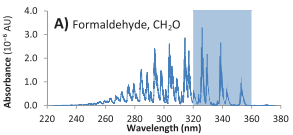
\includegraphics{Figures/HCHO/HCHOAbsorbanceDavenport.png}
      \caption{ %
        HCHO spectrum, with a typical band of wavelengths used for DOAS path measurements.
        This is a portion of an image from \textcite{Davenport2015}.}
      \label{LR:HCHO:Measurements:fig_HCHOSpectrum}
    \end{figure}
    
    FTIR and DOAS measurements have a range of uncertainties, including systematic and random measurement errors and uncertain a priori shape factors and water profiles (eg: \textcite{Franco2015}).
    Other types of measurement involve directly measuring the air, and determining chemical compounds through their physical properties such as by mass spectrometry analysis of mass to charge ratios ($m/z$) of ionised air masses.
    Two examples of this include proton transfer reaction mass spectrometers (PTR-MS), and gas chromatography mass spectrometers (GC-MS).
    These instruments can be used to determine gas phase evolution of isoprene and monoterpene products such as HCHO \parencite[eg.][]{Lee2006a,Nguyen2014,Wolfe2016,Lerner2017}.
    %\textcite{Nguyen2014} use and compare several instruments (including one which is PTR-MS based) in the analysis of isoprene and monoterpene products.
        
    Other measurement techniques include chromatographic and fluorimetric methods, both of which differ widely from each other and the spectroscopic methods \parencite{Hak2005}.
    \textcite{Hak2005} examine a single air mass with 8 instruments using the four techniques (MAX-DOAS, FTIR, chromatographic, and flourimetric), and show that reasonable agreements can be achieved.
    Generally the measurements were close, the five Hantzsch instruments agreeing to within 11\% (after removing two potentially faulty measurements), although different calibration standards were used.
    Titration for the different calibration solutions could not be resolved, which may account for absolute offsets up to 30\%.
    These differences and non-uniformities between measurements (even among identical instruments) are part of the reason HCHO does not have a consistent network for global measurements like those for greenhouse gases or ozone \parencite{FortemsCheiney2012}.
  
    \subsubsection{Satellite measurements}
      \label{LR:HCHO:Sat}
      
      % How satellites give us Vertical Columns and what is AMF
      Satellites remotely sense atmospheric HCHO through irradiance measurements of solar light which has reflected off the earth's surface. 
      These irradiances are affected by gases which exist along the reflected path of light between the detector, earth, and sun. 
      The irradiance is then used to estimate how much of a particular gas exists along this path, which gives us an estimate which is called a slant column (SC).
      The retrieved SC of a particular gas (or species) can be transformed into a vertical column (VC) by scaling the path length in conjunction with accounting for the trace gas' light scattering properties.
      The scaling coefficient created to transform from SC to VC is called the Air Mass Factor (AMF).
      
      Several satellites provide long term trace gas observations with near complete global coverage, including the ERS-2 launched in April 1995 which houses the GOME ultraviolet and visible (UV-Vis) spectrometer, the AURA launched in July 2004 which houses the OMI UV-Vis spectrometer, the MetOp-A and B launched in October 2006 and September 2012 respectively both housing a GOME-2 UV-Vis spectrometer.
      These satellites are on Low Earth Orbit (LEO) trajectories and overpass any area up to once per day.
      Satellites use DOAS techniques with radiative transfer calculations on solar radiation absorption spectra to measure column HCHO .
      An example of a spectrum retrieved from the GOME-2 instrument is given in figure \ref{LR:HCHO:Sat:fig_GOME_products}.
      
      \begin{figure}
        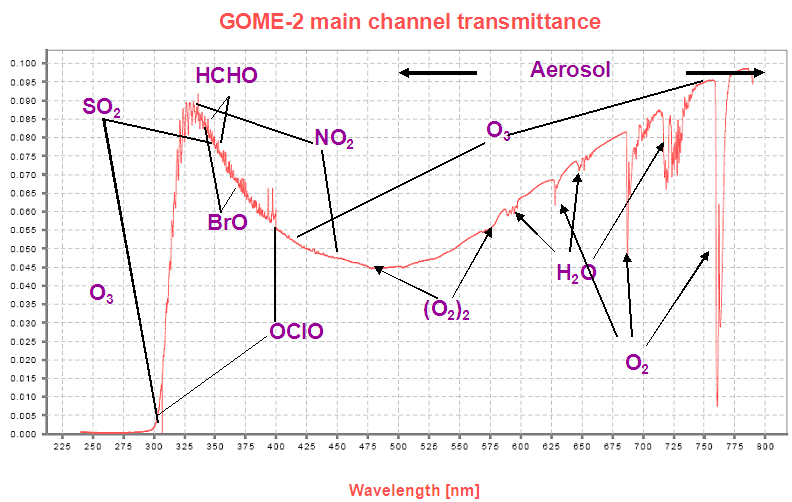
\includegraphics[width=\textwidth]{Figures/GOME_SPECTRUM.jpg}
        \caption{%
          An example spectrum showing interferences used for species concentration measurements by GOME-2. Image by EUMETSAT and ESA \parencite{GOME2Image}.
          }
        \label{LR:HCHO:Sat:fig_GOME_products}
      \end{figure}
      
      % Lead in to modelling
      In conjunction with atmospheric chemistry and radiative models, satellite measurements quantify the abundance of HCHO in the atmosphere.
      Isoprene is hard to measure directly due to its short lifetime and weak spectral absorption, instead HCHO is often used as a proxy \parencite{Millet2006, Fu2007, Dufour2009, Marais2012, bauwens2013satellite, Kefauver2014, Bauwens2016, Surl2018}.
      This leads to a method of isoprene emissions estimation termed top-down (as opposed to bottom-up estimates).
      The existence of satellite data covering remote areas provides an opportunity to improve VOC emissions estimates leading to more robust models of global climate and chemistry. 
      Satellite data gives us another way to estimate large scale isoprene emissions, and their subsequent chemistry.
      This method is described in detail in section \ref{BioIsop:Methods}.
  
\section{Atmospheric Chemistry Modelling}
\label{LR:Models}
  
  Models can fill the gaps (both spatial and temporal) in measurement records, and can help us improve our understanding of the natural world.
  They are used to examine future outcomes resulting from changing our emissions, from small to large scales.
  They can be used to increase measurement accuracy (for instance in satellite measurements) and determine where we lack information, while also checking the performance of new instruments.
  Precisely representing various chemicals and reactions in the atmosphere allows efficient mitigation of pollution, since we can compare scenarios against one another.
  Models can always be expanded to include new compounds or processes, however validation is always necessary.
  Currently they require improved isoprene emissions and subsequent chemistry understanding for effective air quality determination \parencite{Marvin2017}.
  
  \subsection{Box models}
    Box models are much smaller scale than global CTMs, examining one uniform environment with many parametrisations such as transport and emissions.
    Box models can be used to check chemical mechanisms in specific scenarios, such as high or low NO$_X$ environments.
    For example: \textcite{Marvin2017} use a box model matching conditions in southeast USA to evaluate isoprene mechanisms from several models.  
    A box model involves modelling chemistry in a singular set of conditions without transport or any spatial gradients.
    %One box model used in this thesis is called CAABA/MECCA, and is described in Section \ref{Model:CM}.
    
    By allowing for interactions between boxes this concept can be extended to multiple-box models.
    These are simply multiple instances of single boxes with the addition of transport between them, which requires meteorological fields such as wind velocities and turbulence.
    The meteorology fields can be modelled, and/or input as parameters.
  
  
  \subsection{Chemical transport models}
    \label{LR:Models:ctm}
    Chemical transport models (CTMs) provide a simulation of chemical densities and transport over time, through the atmosphere.
    They require many inputs (such as wind velocities) in order to accurately represent scenarios or regions on earth.
    Models of emissions are often used as drivers for atmospheric chemistry models, which require initial and boundary conditions in order to run.
    Chemistry in the atmosphere is a complex system of coupled reactions and dynamics, which can be solved using numerical partial differential equation solvers.
    
    CTMs simulate production, loss, and transport of chemical species.
    This is generally calculated using one or both of the Eulerian (box) or Lagrangian (puff) frames of reference.
    Eulerian models use examine equations and transport within and between volumes in a spatial coordinate systems, while Lagrangian models look at behaviour within a potentially changing frame of reference (for example within a cloud).
    CTMs normally solve continuity equations simultaneously for many coupled species.
    The continuity equations describe transport of a conserved quantity such as mass or energy, which, solved together with production and loss of a chemical can provide detailed simulations of natural processes.
    
    The general continuity equation links a quantity of a substance (q) to the field in which it flows and can be described by the formula:
    \begin{align*}
      \frac{\partial \rho}{\partial t} + \nabla \cdot j = \sigma 
    \end{align*}
    where $\rho$ is density of q in the field, t is time, $\nabla$ is divergence, j is the flux (q per unit area per unit time entering or leaving the field), and $\sigma$ is the generation or loss of q per unit volume per unit time.
    
    
    The type of model best suited to modelling the entire earth uses the Eulerian frame of reference, where the atmosphere is broken up into 3-D boxes with densities and transport calculated and stored for sequential steps in time at each location.
    The mass balance equation must be satisfied in any realistic long term model and is as follows: 
    \begin{align*}
      \frac{dm}{dt} & = \sum{sources}-\sum{sinks} \\
                    & = F_{in} + E + P - F_{out} - L - D 
    \end{align*}
    where m is mass of a chemical, E and D are emission and deposition, P and L are production and loss, and F is chemical transport in and out, as shown in figure \ref{LR:Models:fig_boxmodel}.
    Many chemical species interact with each other through production and loss. 
    Any large chemical model will solve this mass balance equation over highly coupled arrays of partial differential equations, which becomes computation time expensive as complexity increases.
    
    \begin{figure}
      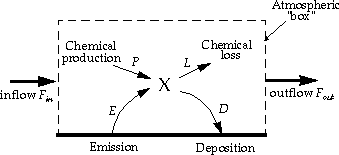
\includegraphics{Figures/boxmodel.png}
      \caption{ %
        Standard box model parameters, image taken from \textcite{Jacob_1999_book}. }
      \label{LR:Models:fig_boxmodel}
    \end{figure}
    
    Contemporary models generally use mathematical differential solving tools of various complexity (often called chemical mechanisms) to solve chemical equations in order to predict chemical species evolutions over time.
    Different solvers may be slower or faster and more suited to particular situations based on the stability of the equations and systems involved, and chemical mechanisms may vary in how many reactions and chemicals are listed and grouped together.
    For example: Since [O] $<<$ [O$_3$] the chemical family O$_X$ (  O$_X \equiv $ O $+$ O$_3$ ) can be used to simplify chemistry simulations and approximate O$_3$ concentrations \parencite[][Chapter 3]{BrasseurJacob2017}.
    Different chemical mechanisms may find different solutions to the same problems, due to how the numerical solvers are implemented, which can affect model output \parencite{Zhang2012}.
    %\textcite{Zhang2012} examine the outputs from a regional model (WRF/Chem) using three different chemical mechanisms, and they show some model output sensitivity to the choice of mechanism.
    %particulate matter prediction is sensitive to the choice of chemical mechanism. 
    
  
  \subsection{Emissions}
  
    %% HOW estimates are made
    There are two commonly used ways of estimating isoprene emissions, top-down or bottom-up.
    Bottom-up emission estimates generally model the flora which emit isoprene, along with the rates of emissions and things which affect these rates.
    The general formula governing modelled emissions $E$ for a species $i$ (from \textcite{BrasseurJacob2017}) is as follows:
    \begin{equation*}
      E_i = A \times EF_i \times S_i
    \end{equation*}
    with $A$ the activity rate (eg. how many trees in an area), $EF_i$ being the emission factors (eg. isoprene emitted per tree per year), and $S_i$ is a scaling factor accounting for meteorology and other effects not included in $A$ or $F$ (eg. seasonal temperature).
    
    
    Isoprene is emitted by trees or shrubs, depending on several parameters such as leaf area index (LAI), plant functional type (PFT), and light density fraction (LDF).
    Models use these properties of the emitters in order to estimate how much isoprene is being produced \parencite[eg.][]{Guenther1995,Guenther2006}.
    Understanding how much isoprene is emitted, when and by what, is complicated.
    One frequently used bottom up emissions model is the Model of Emissions of Gases and Aerosols from Nature (MEGAN, \textcite{Guenther1995}).
    MEGAN has estimated $\sim 1150$\tgcpyr BVOC emissions globally, of which $\sim$465-500\tgcpyr is isoprene \parencite{Guenther2006, Messina2016}. 
    Since little data exists with which to verify these bottom-up emission inventories, they can be uncertain on a large scale.
    
    %In many CTMs the isoprene emissions are calculated seperately (for example by running MEGAN), and then used as boundary conditions \parencite[eg.][]{Guenther2006}. 
    %This can speed up calculations as the transport and concentrations can be simulated in various conditions without recalculating the emissions.
    %Trace gases with short lifetimes and complex chemistry such as isoprene are often hard to measure which makes verifying model estimates difficult.
    
    % how bottom up models are sensitive:
    Bottom up models of VOC emissions are sensitive to parameters.
    For example \textcite{Stavrakou2014} examined modelled Asian emissions and altered model parameters for temperature, plant type emission factors, incoming solar radiation (insolation) intensity, land use changes, and palm tree forest expansion.
    Changes were constrained by a network of radiation measurements and some experiments with south east Asian forest emissions - and led to reduction in a priori isoprene emissions by a factor of two over the region in 2005.
    Sensitivity to these factors is pervasive in bottom up emissions models \parencite[eg.][]{Marais2014,Miller2014,Messina2016}.
    One of the important uncertainties seen in MEGAN is the isoprene emissions due to PFTs.
    %Canopy level isoprene measurements are made using relaxed eddy accumulation at several sites in Africa.
    If one plant species is emitting heavily near a measuring instrument, possible overestimations may occur due to extrapolation over the entire forest.
    Global emissions inventories like MEGAN often have large areas based on extrapolations which introduces uncertainties \parencite{Miller2014}.
    Current emissions estimates require more validation against observations, and recently a comparison of two major VOC models (MEGAN and ORCHIDEE) was undertaken by \textcite{Messina2016} reiterating this requirement.
    In their work they examine model sensitivities and show that the most important parameters are LAI, EF, PFT, and LDF.
    There is high uncertainty in LAI and EF, which require more or improved measurements at the global scale, as well as more PFTs and improved LDF parameterisation \parencite{Messina2016}.
    
  
  \subsection{Uncertainties}
  \label{LR:Models:Uncert}
    
    Here I will attempt to list and partially explain the major uncertainties models have in relation to  VOCs, and ozone.
    Atmospheric chemical models by necessity require various simplifications of real world processes, and also utilise information which may be itself uncertain or extrapolated.
    Uncertainty is introduced through both of these channels as well as through computational limitations and non-linear non-continuous system solution approximations.
    
    
    \subsubsection{Emissions Inventories}
      % Emissions Inventories 
      Using different emissions inventories in a CTM can have large impacts on the simulation.
      Natural (biogenic or pyrogenic) and human driven (anthropogenic) emissions often drive a large fraction of atmospheric oxidation and radical chemistry, especially in the continental boundary layer.
      Emissions inventories have been found to be generally OK at larger (regional to global) scales, as long as they are derived from accurate input measurements \parencite{Zeng2015}.
      Modelled ozone concentrations has been found to be most sensitive to isoprene emissions and NO$_X$ sources, both of which have uncertainty factors of $\sim 2$ \parencite{Christian2017}.
      
      Many estimates of isoprene emission are based on a few algorithms which can depend greatly on input parameters \parencite{Arneth2008,Niinemets2010}.
      \textcite{Arneth2008} argue that this monopoly of emissions estimates may be leading us to an incorrect understanding of isoprene chemistry.
      \textcite{Yue2015} have shown that this is still a problem by looking at land carbon fluxes and modelling the sensitivity to VOC emissions estimates using two independent models of VOC emission.
      One model is photosynthesis based and estimates isoprene emissions using electron transfer energies and leaf physiology \parencite{Niinemets1999}, while the other (MEGAN) uses the light and canopy temperature \parencite{Guenther1995,Arneth2007}.
      % Arneth et al., 2007; CO2 may also inhibit isoprene emissions.
      % Unger et al., 2013; another plant process isoprene model
      Both are sensitive to light and temperature parameterisations.
      
      The concentration of NO$_X$ is an important factor in determining the yield of HCHO and ozone from BVOCs.
      \textcite{Travis2016} show how modelled surface ozone is overestimated due to high estimates of NO$_X$ emissions, which affect oxidative capacity and VOC reactions in the US.
      NO$_X$ and isoprene emissions are shown to be the most significant sources of uncertainty for ozone concentrations near the surface in GOES-Chem over the US, while isoprene derived products and lightning NO$_X$ drives uncertainty in the upper atmosphere \parencite{Christian2017}.
      
    %% GEOS-Chem resolution uncertainties
    \subsubsection{Resolution}
      \label{LR:Models:Uncert:Resolution}
      
      Atmospheric chemistry simulations are somewhat sensitive to the gridbox resolution.
      For example: \textcite{Wild2006} show that reduced resolution increases OH concentrations and ozone production rates.
      \textcite{Christian2017} find small changes in OH ($<10$\%) in OH, HO$_2$ and ozone concentrations local to the north American arctic, when changing from 4 by 5 to 2 by 2.5\degr resolution.
      \textcite{Yu2016} show how only at higher resolution (0.25 by 0.3125\degr) does isoprene oxidise under the correct NO$_X$ scheme (through high or low NO$_X$ pathways, see section \ref{LR:VOCs:IsopCascade:Oxidation}) in variable NO$_X$ environments.
      This leads to an increase of high NO$_X$ pathway oxidation of isoprene at the lower resolutions, which leads to an overestimation of HCHO but not ozone at coarser resolutions.
      However, for many global scale analyses, errors from resolution are less important than those from chemistry, meteorology, and emissions \parencite{Christian2017, Christian2018}.
      
            
    
    \subsubsection{Chemistry mechanisms}
      \label{LR:Models:Uncert:Chemistry}
      %% GEOS-Chem Ozone uncertainties 
      There is still much work to be done in models to correctly simulate emissions and processes which lead to HCHO and ozone.
      Often HCHO is used as a way of checking if precursors are correctly modelled since HCHO measurements are more readily available (for instance from satellites).
      Recently \textcite{Christian2017} analysed GEOS-Chem (A global CTM; see section \ref{Model:GC}) for ozone and oxidant (OH and HO$_2$) sensitivity to the driving processes and inputs.
      They found that GEOS-Chem ozone was most sensitive to NO$_2$ photolysis, the $NO_2 + OH$ reaction rate, and precursor emissions such as VOCs.

      Many models lack in-situ measurements with which to verify their chemical mechanisms, leading to large discrepancies \parencite{Marvin2017}.
      \textcite{Marvin2017} suggest that isoprene mechanisms in several contemporary models (including GEOS-Chem) are inadequate. 
      They show that (for a specific measurement campaign) HCHO concentrations are underestimated in a way that can not be easily fixed through reaction rate changes.
      They compared five global CTMs isoprene mechanisms by evaluating simulated HCHO mixing ratios compared to in situ measurements from the Southeast Nexus (SENEX) aircraft campaign (in southeastern USA).
      Five models (GEOS-Chem, CB05, CB6r2, MCMv3.2, and MCMv3.3.1) all are found to underestimate HCHO concentrations (by $15 - 30\%$).
      
    
    \subsubsection{Clouds}
      \label{LR:Models:Uncert:Clouds}
      One of the major uncertainties in chemical, climate, radiation, and weather models is cloud formation and dynamics.
      Clouds are remarkably complex at a much finer scale than can be accurately modelled by global chemistry models (with current processing power).
      Globally over half (50-60\%) of the world is covered by clouds, with $\sim10\%$ of them being rain-clouds \parencite{Kanakidou2005}.
      Wet scavenging performed in clouds not only depends on large scale cloud processes, but also on the microphysics of aerosols being scavenged, differing between aerosol sizes and hygroscopic properties.
      
      
    
    \subsubsection{Soil Moisture}
      \label{LR:Models:Uncert:SoilMoisture}
      Modelled emissions are sensitive to soil moisture, especially near the wilting point, below which trees stop emitting isoprene and other VOCs completely as they can no longer draw water \parencite{Bauwens2016}.
      MEGAN accounts for soil moisture through a parameterisation which drops plant emissions to zero below a prescribed soil moisture level (the wilting point).
      Recently an update to this has been shown to improve modelled isoprene emissions in drought conditions \parencite{Jiang2018}.
      \textcite{Jiang2018} found that improving the parameterisation of drought based on a measurement campaign in the U.S. would lower isoprene emissions globally by $\sim17\%$.
      Many environmental parameters are affected by soil moisture, which all play a role at fine scales to surface emissions \parencite{Rowntree1983,Chen2001}.
      %\textcite{Rowntree1983} show how quickly soil moisture anomalies affect rainfall and other weather systems, while \textcite{Chen2001} specifically show how important fine scale soil moisture information is when modelling land surface heat flux, and energy balances.
      Droughts effects can be difficult to measure, as they are a multi-scale problem which affects various aspects of the land-air interface including plant emissions and dry deposition \parencite{Wang2017}.
      

\section{Australia and the southern hemisphere}
\label{LR:Aus}
  
  % Description of uniqueness
  Australia has a unique climate, along with soil moisture, clay content and other important properties which affect VOC emissions.
  These properties are only sparsely measured in Australia due to the spread out distribution of population centres, which make many areas very difficult or expensive to reach.
  In Australia most long term air quality or composition measurements are performed in or near large cities.
  Australia is dominated by areas with little anthropogenic influence and few ground based measurements of the natural emissions taking place \parencite{VanDerA2008}.
  Since many Australian cities are on the edge of regions with rich VOC emissions, it is very important to clarify the quantity, type, and cause of VOC emissions.
  Understanding of emissions from these areas is necessary to inform national policy on air pollution levels.
  
  The vegetation in Australia is diverse, a summary is provided by ABARES using the national forest inventory at  \url{http://www.agriculture.gov.au/abares/forestsaustralia/australias-forests}.
  Figure \ref{LR:Aus:fig_forests} shows the different forest types and their locations within Australia, highlighting that much of our forested lands are near population centres along the east coast.
  16\% of Australia is covered by forest, most (75\%) of which is Eucalyptus.
  
  \mypic{Figures/ForestTypes.png}{Forest types in Australia (\url{http://www.agriculture.gov.au/abares/forestsaustralia/australias-forests})}{\label{LR:Aus:fig_forests}}
  
  %Transport stuff
  Ozone enhancements above the background levels are most sensitive to emissions (of precursor gases), with meteorology, and atmospheric composition also important.
  Anthropogenic emissions of ozone precursors are important but relatively stable, while pyrogenic sources are greatly variable and dependent on weather, fuel, and fire intensity \parencite[e.g.][]{Lawson2017}. 
  Emissions from burning include a range of chemical compounds and particulates and each year the effects of fire or burning seasons blanket the northern and southern hemispheres independently.
  Biomass burning in southern Africa and South America has previously been shown to have a major influence on atmospheric composition in Australia \parencite{Oltmans2001, Gloudemans2006, Edwards2006}, particularly from July to December \parencite{Pak2003, Liu2016}.
  Local fires are even more influential and the burning season for Australia can be all year, with severity depending on regional vegetation, recent and current weather, and El-ni$\tilde{n}$o.
  
  
  % Australia could be a VOC hotspot
  It has been estimated by MEGAN that the Australian outback is among the world's strongest isoprene emitters with forests in SE Australia having emission factors greater than 16 mg m$^{-2}$ h$^{-1}$ (see figure \ref{LR:Aus:fig_MEGAN_EF}) \parencite{Guenther2006,Guenther2012}.
  Measurement campaigns in SE Australia have since cast doubt on the emission factors used by MEGAN, potentially due to poor characterisation of Eucalyptus trees and soil moisture \parencite{Emmerson2016}.
  These emissions factor estimates are not well verified and measurements of isoprene (or other BVOC) emissions are sparse and infrequent in Australia \parencite{Sindelarova2014, Bauwens2016}.
  In addition, monoterpene emissions are 2-4 times too low, which may be due to underestimated emission rates for many Eucalypt species \parencite{Winters2009,Emmerson2016}.

  \begin{figure}
    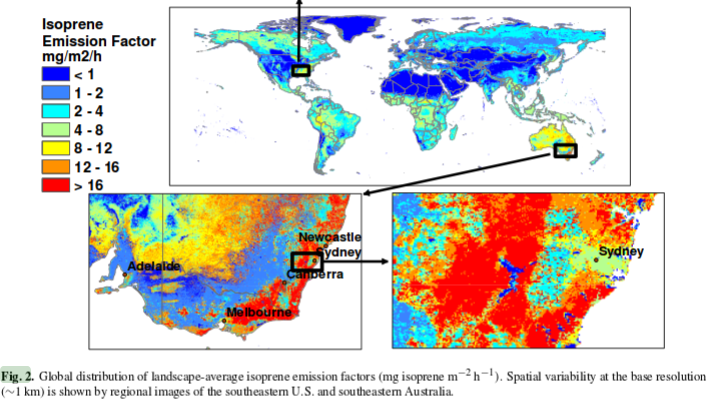
\includegraphics[width=\textwidth]{Figures/MeganIsoprene1.png}
    \caption{ Part of a figure from \textcite{Guenther2006} showing global isoprene emission factors. }
    \label{LR:Aus:fig_MEGAN_EF}
  \end{figure}
  
  
  \subsection{Ozone}
    Surface ozone levels over Australia are relatively low ($\sim20$~ppb) \parencite{Young2018}, however it remains unclear how much we would expect this to change in the future as relatively little is known about precursors and influx for the continent.
    % Air Quality metric example
    Australian air quality is monitored independently within each state, using several metrics.
    These metrics are measured by varying numbers of monitoring stations in each state.
    %In New South Wales (NSW) the metrics used to determine air quality are: particulate matter (PM), O$_3$, CO, NO$_2$, SO$_2$, and visibility.
    %An air quality index equal to the worst of these metrics is used for NSW as shown at \url{http://www.environment.nsw.gov.au/aqms/aqitable.htm}.
    %Similar methods are used in other states to get an idea of air quality.
    Measurement stations are generally located in population centres, and do not regularly measure isoprenoid emissions. 
    This is an important omission as these naturally emitted precursor gases often get transported into cities where they affect air quality through production of O$_3$ and other pollutants.
    
    Generally STT of ozone over Australia affects the upper troposphere only, however ozone enhancements can reach quite low during heavy storms and cyclonic weather patterns \parencite{Alexander2013}.
    The contribution of STT to overall tropospheric ozone budgets remains uncertain, especially in the southern hemisphere (SH) \parencite{Skerlak2014}.
    STT can enhance surface ozone concentrations above legal air quality limits \parencite[e.g.][]{Lelieveld2009,Lin2015}.
    It is easier to determine tropospheric ozone enhancements over the relatively clean southern ocean atmosphere.
    However measurements of tropospheric ozone over this region are relatively sparse \parencite{Skerlak2014}, and quantification of transported ozone is difficult without large scale extrapolations.
    Ozone enhancements over the southern ocean signify either transported pollution or stratospheric influx \parencite{Jacobson2000}.
    Quantifying ozone processes over the southern ocean would be helpful towards understanding chemistry in the ``clean background environment'', which is important when validating models and satellite datasets.
  
  % voc estimates
  \subsection{VOCs}
    
    % Vocs are uncertain because...
    Bottom up inventories of VOCs remain largely uncertain due to extensive extrapolation over plant functional types, changing land cover, and parameterised environmental stressors \parencite{Guenther2000,Kanakidou2005,Millet2006}.
    \textcite{Muller2008} show how isoprene (a key VOC) is poorly captured by the MEGAN model and analyse the affect of changing the soil moisture parameter.
    \textcite{Sindelarova2014} show reductions in modelled Australian isoprene emissions of 50\% when incorporating soil moisture in MEGAN estimates. 
    Uncertainties in isoprene emissions could explain why models of HCHO over Australia are poor at reproducing satellite measurements \parencite{Stavrakou2009}.
    Improved parameterisation of the affect of drought on plant emissions could also lower modelled isoprene emissions \parencite{Jiang2018}.
    
    
    % Australian VOCs suffer even specifically from:
    Australia suffers from poor characterisation of plant emissions, partly because emission factors are based on northern hemispheric data.
    Many plant emissions rates have not been published, such as those for any Australian acacias.
    Some Eucalypt emissions are based on samples from young trees, which may emit more isoprene than older trees \parencite{Emmerson2016}.
    Additionally soil moisture is not well quantified which has a large effect on emissions.
    Soil type and moisture, along with drought threshholds, have poorly understood effects on plant emissions in Australia
    Changes in parameterisation of soil moisture in the MEGAN lead to massive changes in Australian isoprene emission estimates \parencite{Sindelarova2014}.
    Over Australia MEGAN suffers from a lack of studied plant functional types and their emissions \parencite[eg.][]{Muller2008}.
    Emission rates from various species of Eucalyptus and other flora are highly complex, depending on current and recent weather, temperature, tree age, health, etc. \parencite{Guenther2012}. 
    With this complexity added to the diversity of tree species in Australia as well as sparse rural data collections it is hard to model and verify emissions.
       
    % What did Emmerson do?
    \textcite{Emmerson2016} %analyse EF sensitivity of a high resolution model of atmospheric chemistry over southeast Australia, comparing isoprene and monoterpene emissions against 4 separate campaigns.
    analysed isoprene and monoterpene emissions sensitivities in a regional model of atmospheric chemistry over southeast Australia, using four campaigns which are also examined in this thesis.
    They show that modelled emissions require spatially and temporally resolved changes.
    \textcite{Emmerson2016} suggest that monoterpenes may be emitted in similar quantites to isoprene, with more measurements required to determine if this is so.
    They compare emissions estimates from MEGAN against field campaign data and see overestimated isoprene emissions, as well as underestimated monoterpene emissions.
    Their work suggests that MEGAN estimates of isoprene emissions may be 2-6 times too high, and monoterpene emissions $\sim3$ times too low over southeast Australia.
    
    
    % How could we improve this voc understanding?
    Improvements to emissions models require improved understanding of regions and their behaviour.
    Satellite measurements can be used to improve understanding of Australian emissions.
    As HCHO is produced with relatively high yield after isoprene is emitted, we can use satellite measurements to estimate isoprene emissions \parencite[e.g.]{Palmer2001, Millet2006, Bauwens2016}.
    
  
  \subsection{Measurements}
    
    % Brief overview of all the measurement campaigns.
    Isoprene and many of its products can be difficult to measure accurately due to their short lifetimes, high reactivity, and optically thin natures.
    There are relatively few measurements in the southern hemisphere, including MUMBA \parencite{PatonWalsh2013}, SPS\parencite{Dunne2018}, and Tumbarumba \parencite{Emmerson2016}
    % and that girl from Macquarie University with an instrument in the daintree rainforest(CITE,describe if available before finished).
    These campaigns focus on air quality or biogenic emissions and use several different instruments (including PTR-MS and GC-FID) to detect metrics such as air particulates, HCHO, isoprene, and meteorological information.
    An air-flight campaign (HIPPO) measuring over the Pacific ocean, with one flight passing along the NSW coastline, also provides isoprene and ozone concentrations in November 2009 \parencite{Wolfsy2011}.
    Wollongong also has 20 years of DOAS calculated HCHO measurements from a solar FTS. 
    Satellite total columns suffer from orography amongst other limitations when compared to this data \parencite{Demol2010}.
    For further details on these campaigns see Section \ref{Model:Datasets}.
    
    Detecting ozone from the surface up to the top of the stratosphere requires different techniques such as remote sensing and ozonesonde releases.
    Ozonesondes are weather balloons (with attached ozone detectors) which detect ozone concentrations up to the mid stratosphere ($\sim 30$~km), providing a vertical profile over a single location.
    Since 1986, Lauder, New Zealand (45$^{\circ}$S, 170$^{\circ}$E) has released ozonesondes allowing a multi-decadal analysis of ozone concentrations over the city \parencite{Brinksma2002}.
    Kerguelan Island (49.2$^{\circ}$S, 70.1$^{\circ}$E), also has a record of ozonesonde profiles, which are directly in the path of biomass burning smoke plumes transported off shore from Africa \parencite{Baray2012}.
    SHADOZ is the southern hemispheric additional ozone project, which have released sondes from 15 sites at different times \url{http://tropo.gsfc.nasa.gov/shadoz/}.
    A smaller network of ozonesonde release sites (including Davis, Macquarie Island, and Melbourne) is available from the world ozone and ultraviolet radiation data centre \url{http://woudc.org/data/explore.php} and is used in Chapter \ref{Ozone} to examine stratospheric impacts on tropospheric ozone (see \ref{Model:Datasets:ozonesondes} for more info on these ozonesondes).
  
\section{Aims}
\label{LR:Aims}

  \textbf{In this thesis I aim to improve understanding of natural contributions to ozone over Australia and the southern ocean.}
  The two largest contributors to tropospheric ozone concentrations are chemical production (driven by precursor emissions) and stratospheric transport.
  I aim to improve understanding of both of these sources using existing satellite and ground-based datasets along with GEOS-Chem modelled outputs.
  
  % Aim for Chapter 2: Modelling examination
  Estimation of BVOC emissions in Australia can be improved through satellite measurements of one of the primary oxidation products HCHO.
  Satellites which overpass daily record reflected solar (and emitted terrestrial) radiation, and give us measurements over all of Australia.
  Combining satellite data with model outcomes provides a platform for the understanding of natural processes, which are uncertain over Australia.
  Satellite measurements use modelled a priori vertical profiles of HCHO to estimate total column amounts.
  \textbf{I aim to recalculate satellite vertical columns of HCHO using updated model a priori information.}
  In this effort I aim to improving the understanding of the importance of relevant parameters (within GEOS-Chem) in calculating vertical columns of HCHO measured by satellite.
  This includes an examination of how well GEOS-Chem simulates several species such as NO$_X$, isoprene, and HCHO compared to both in-situ and remote measurement data that exists for Australia.
  Additionally I detail the construction and effects of satellite data filters.
  The work towawrds this aim is in Chapter \ref{Model}.
  %Soil moisture plays an important role in VOC emissions, as trees under stress may stop emitting various chemicals. 
  %This is especially true for Australia due to frequent droughts and wildfires.
  %The argument for improved understanding of land surface properties, specifically soil moisture, is an old one\parencite{Mintz1982, Rowntree1983, Chen2001}.
  
  % Aim for Chapter 3: Biogenic emissions estimation
  The technique of determining isoprene emissions from satellite detected HCHO is called satellite inversion.
  \textbf{I aim to determine isoprene emissions in Australia using a top-down inversion of satellite HCHO, through an estimated yield from isoprene to HCHO}
  HCHO amounts and the yield of isoprene to HCHO over Australia is required to create top-down estimates.
  This process also requires careful examination of when the assumptions required within the inversion process are not valid.
  Due to the low availability of in-situ data over most of the Australian continent, a combination of modelled and satellite data could reduce the uncertainties of isoprene emissions from Australian landscapes.
  Improved emissions estimates will in turn improve the accuracy of CTMs, providing better predictions of atmospheric composition and its response to ongoing environmental change.
  The work towards fulfilling this aim is in Chapter \ref{BioIsop}.
  
  % Aim for Chapter 4: STT Ozone
  \textbf{To improve understanding of ozone transported to the troposphere from the stratosphere in Australia and the southern ocean.}
  Stratospheric transport is the second largest driver of tropospheric ozone concentrations, and an improved understanding of transported ozone can be determined from ozonesonde measurements.
  Ozonesondes provide a glimpse of the vertical ozone profile up to $\sim 30$~km, and we use a Fourier filter to determine how often stratospheric transport is occurring at three sites: Melbourne, Macquarie Island, and Davis Station. 
  Combining transport event frequency analysis with modelled ozone distributions is used to derive a new method of detection and quantification of transported ozone in Chapter \ref{Ozone}.
  
  
  % Chapter 5: Conclusions?
  \textbf{I aim to describe relative importance of sources of tropospheric ozone in Australia, as well as seasonality.}
  I will describe how modelled ozone is affected by updated isoprene emissions, comparing changes in GEOS-Chem outputs.
  Trends of isoprene emissions and their relationship to tropospheric ozone trends could provide new insight into the future of tropospheric ozone in Australia.
  
